\subsection{Relevant Sub-systems}

%---------------------- LOCOMOTION ----------------------%

\subsubsection{Locomotion}

Locomotion for ground-based biomimetic robots is usually achieved using a set of animal-like legs.
The following section presents the leg morphologies of various robots in greater detail.

\sssubsection{MiniHyQ} \mbox{}\\

MiniHyQ uses a series-articulated leg morphology \cite{khan_minihyq_2015}.
The upper leg is composed of a folded 1.5mm aluminium sheet while the rest of the leg linkages is milled aluminium parts \cite{khan_development_2015}.
Absolute encoders and torque sensors shown in Figure \ref{fig:minihyq_haa} assist in determining leg position and acceleration.
Figure \ref{fig:minihyq_topology} demonstrates the design.

\begin{figure}[H]
    \centering
    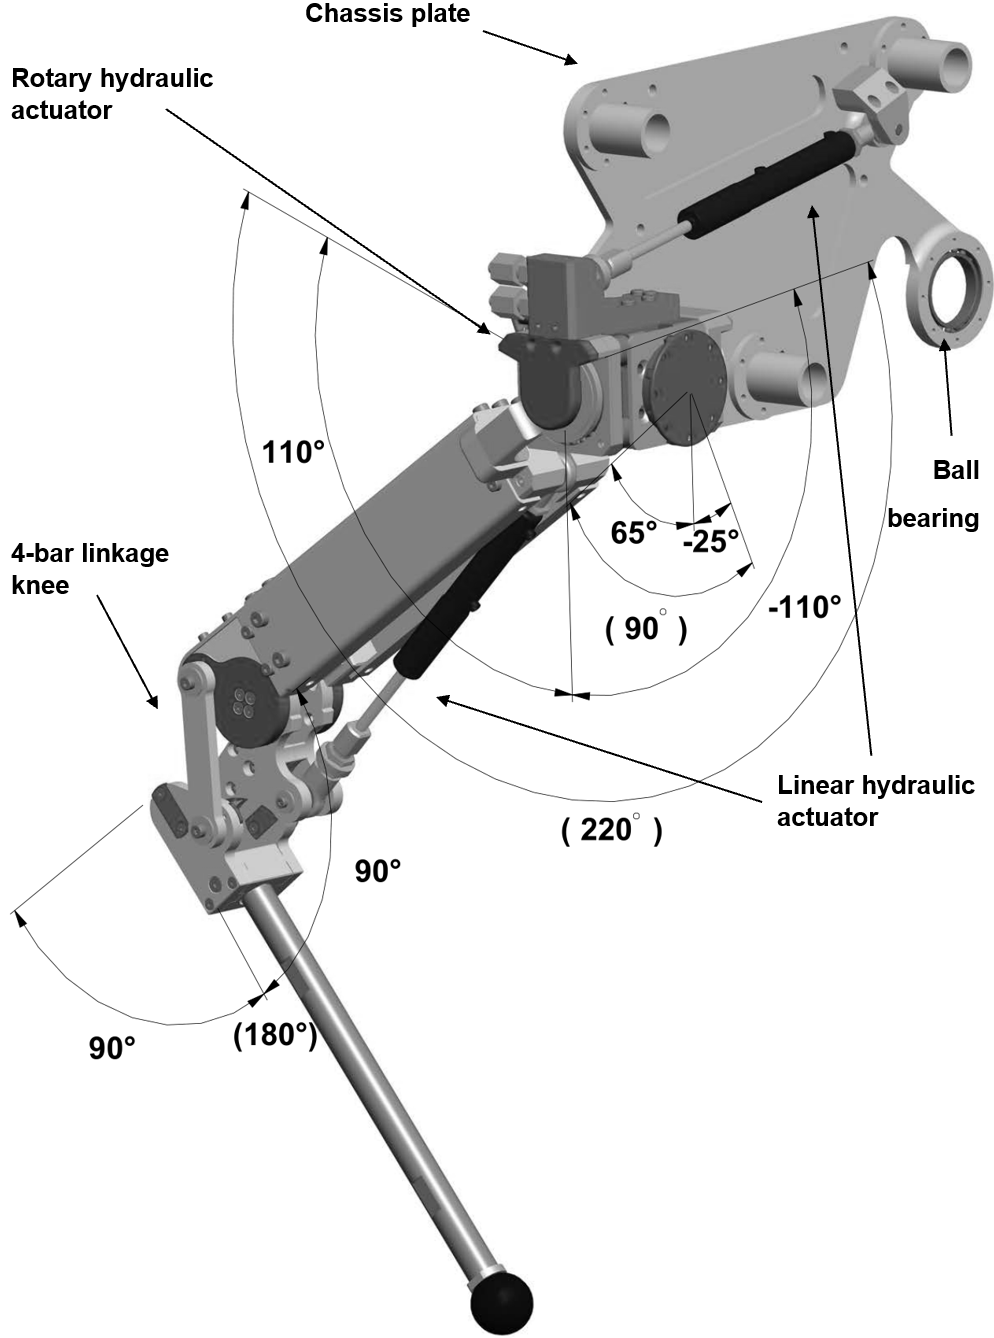
\includegraphics[width=0.6\textwidth]{Sections/LiteratureReview/img/minihyq/subsys_minihyq_topology.png}
    \caption{MiniHyQ Series-articulate leg topology \cite{khan_minihyq_2015}}
    \label{fig:minihyq_topology}
\end{figure}

Hip adduction-abduction, shown in Figure \ref{fig:minihyq_haa}, is actuated via a Fluitronics AZ013 linear hydraulic actuator that connects the chassis to the rotary hydraulic actuator responsible for hip flexion-extension \cite{khan_minihyq_2015}.
The attachment methods are not explicitly stated; it appears to be mounted via bearings to the chassis and rotary actuator.

\begin{figure}[H]
    \centering
    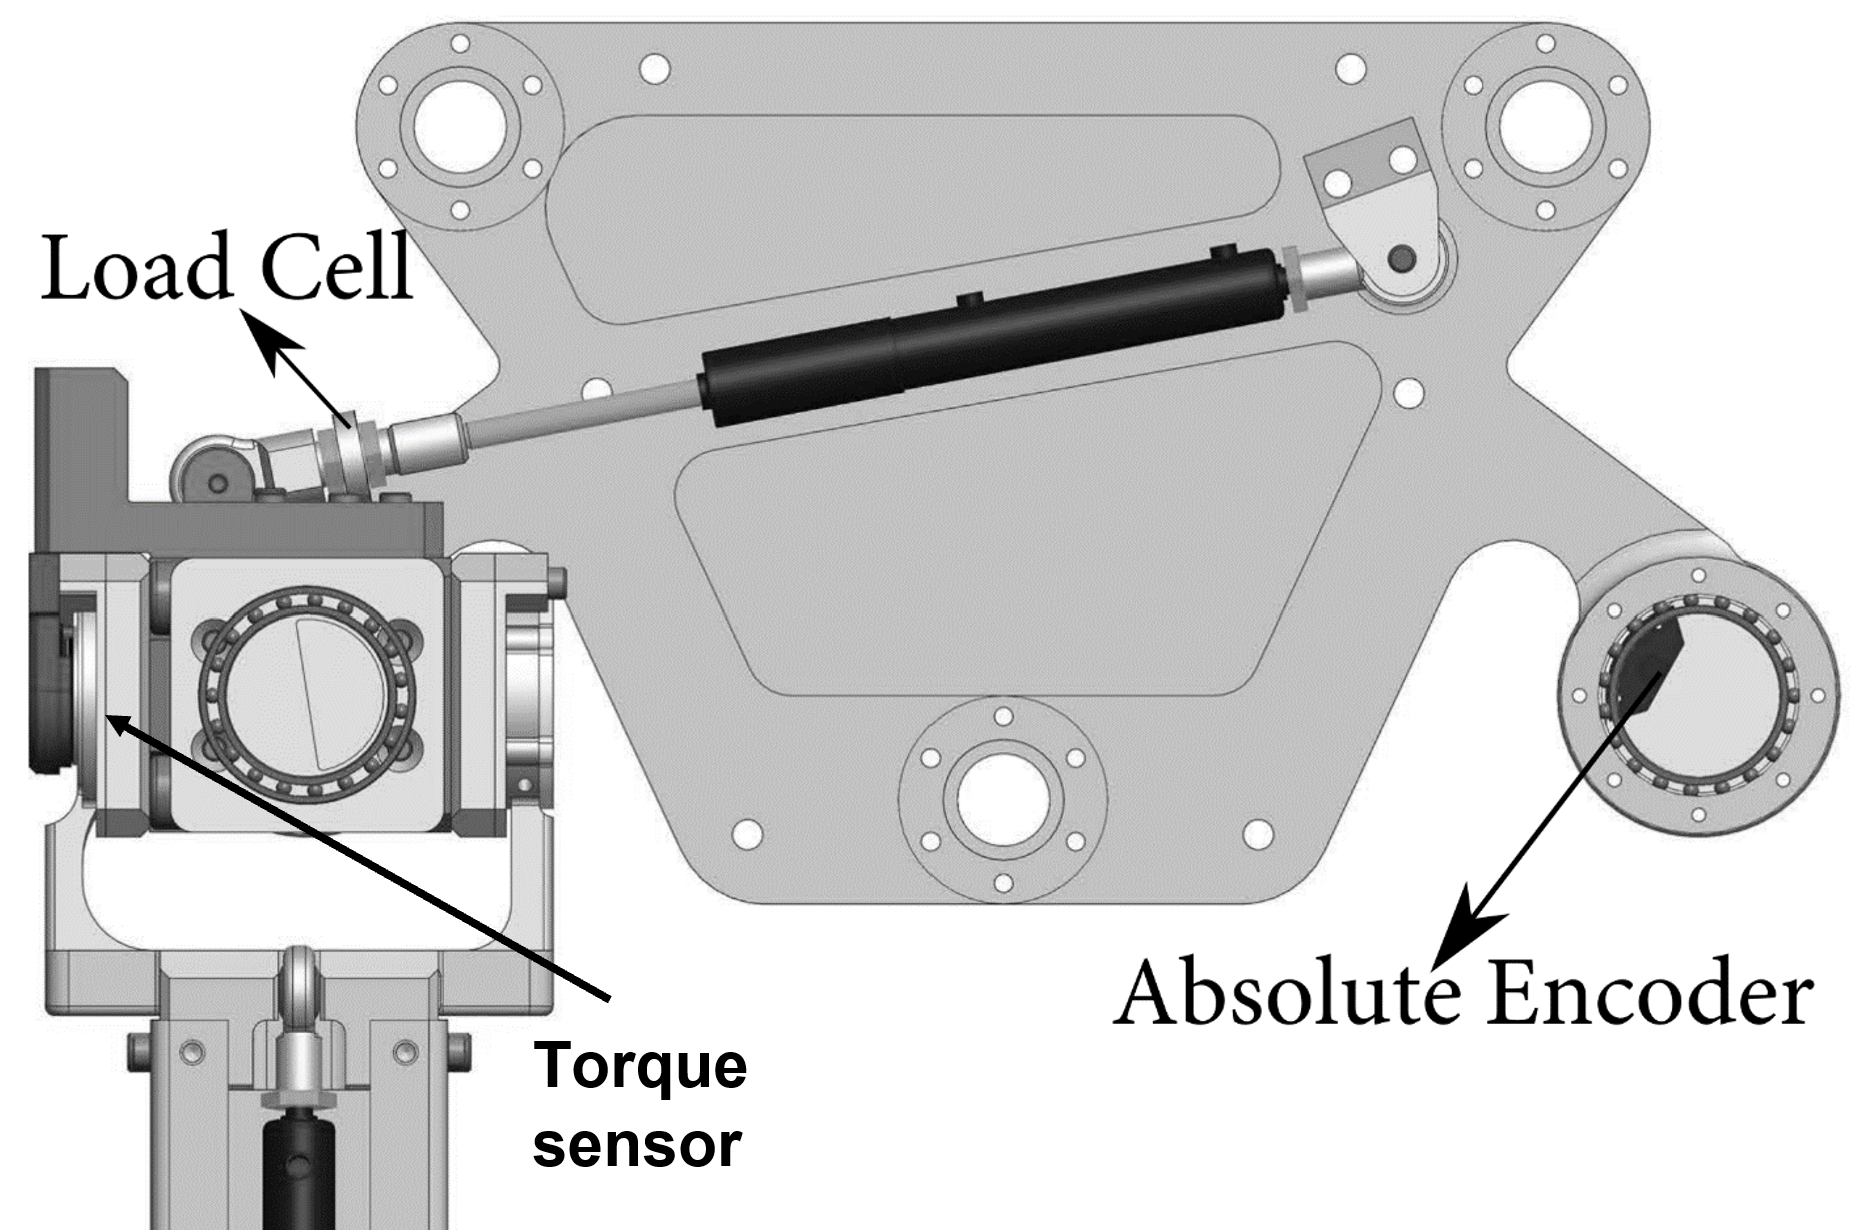
\includegraphics[width=0.6\textwidth]{Sections/LiteratureReview/img/minihyq/subsys_minihyq_haa.png}
    \caption{MiniHyQ Hip abduction and adduction is performed via a linear actuator connecting the chassis to the rotary actuator responsible for flexion and extension \cite{khan_minihyq_2015}}
    \label{fig:minihyq_haa}
\end{figure}

Figures \ref{fig:minihyq_knee_cad} and \ref{fig:minihyq_knee_links} demonstrate the knee linkage when fully extended ($+90^{\circ}$).
The 4-bar configuration shown in Figure \ref{fig:minihyq_knee_cad} allows for a $180^{\circ}$ joint range, superior to the $120^{\circ}$ found on BigDog and other preexisting hydraulically actuated models \cite{khan_development_2015}.
This allows for a greater range of motion and obstacle navigation, as well as the ability to self-right if fallen over. Compared to HyQ, MiniHyQ has a 40\% wider joint range of motion in the sagittal plane.
Although not explicitly stated by the author, individual linkages are likely attached with a set of bushings at the joints, similarly to how it is done with the Stanford Doggo \cite{kau_stanford_2019}.

\begin{figure}[H]
    \centering
    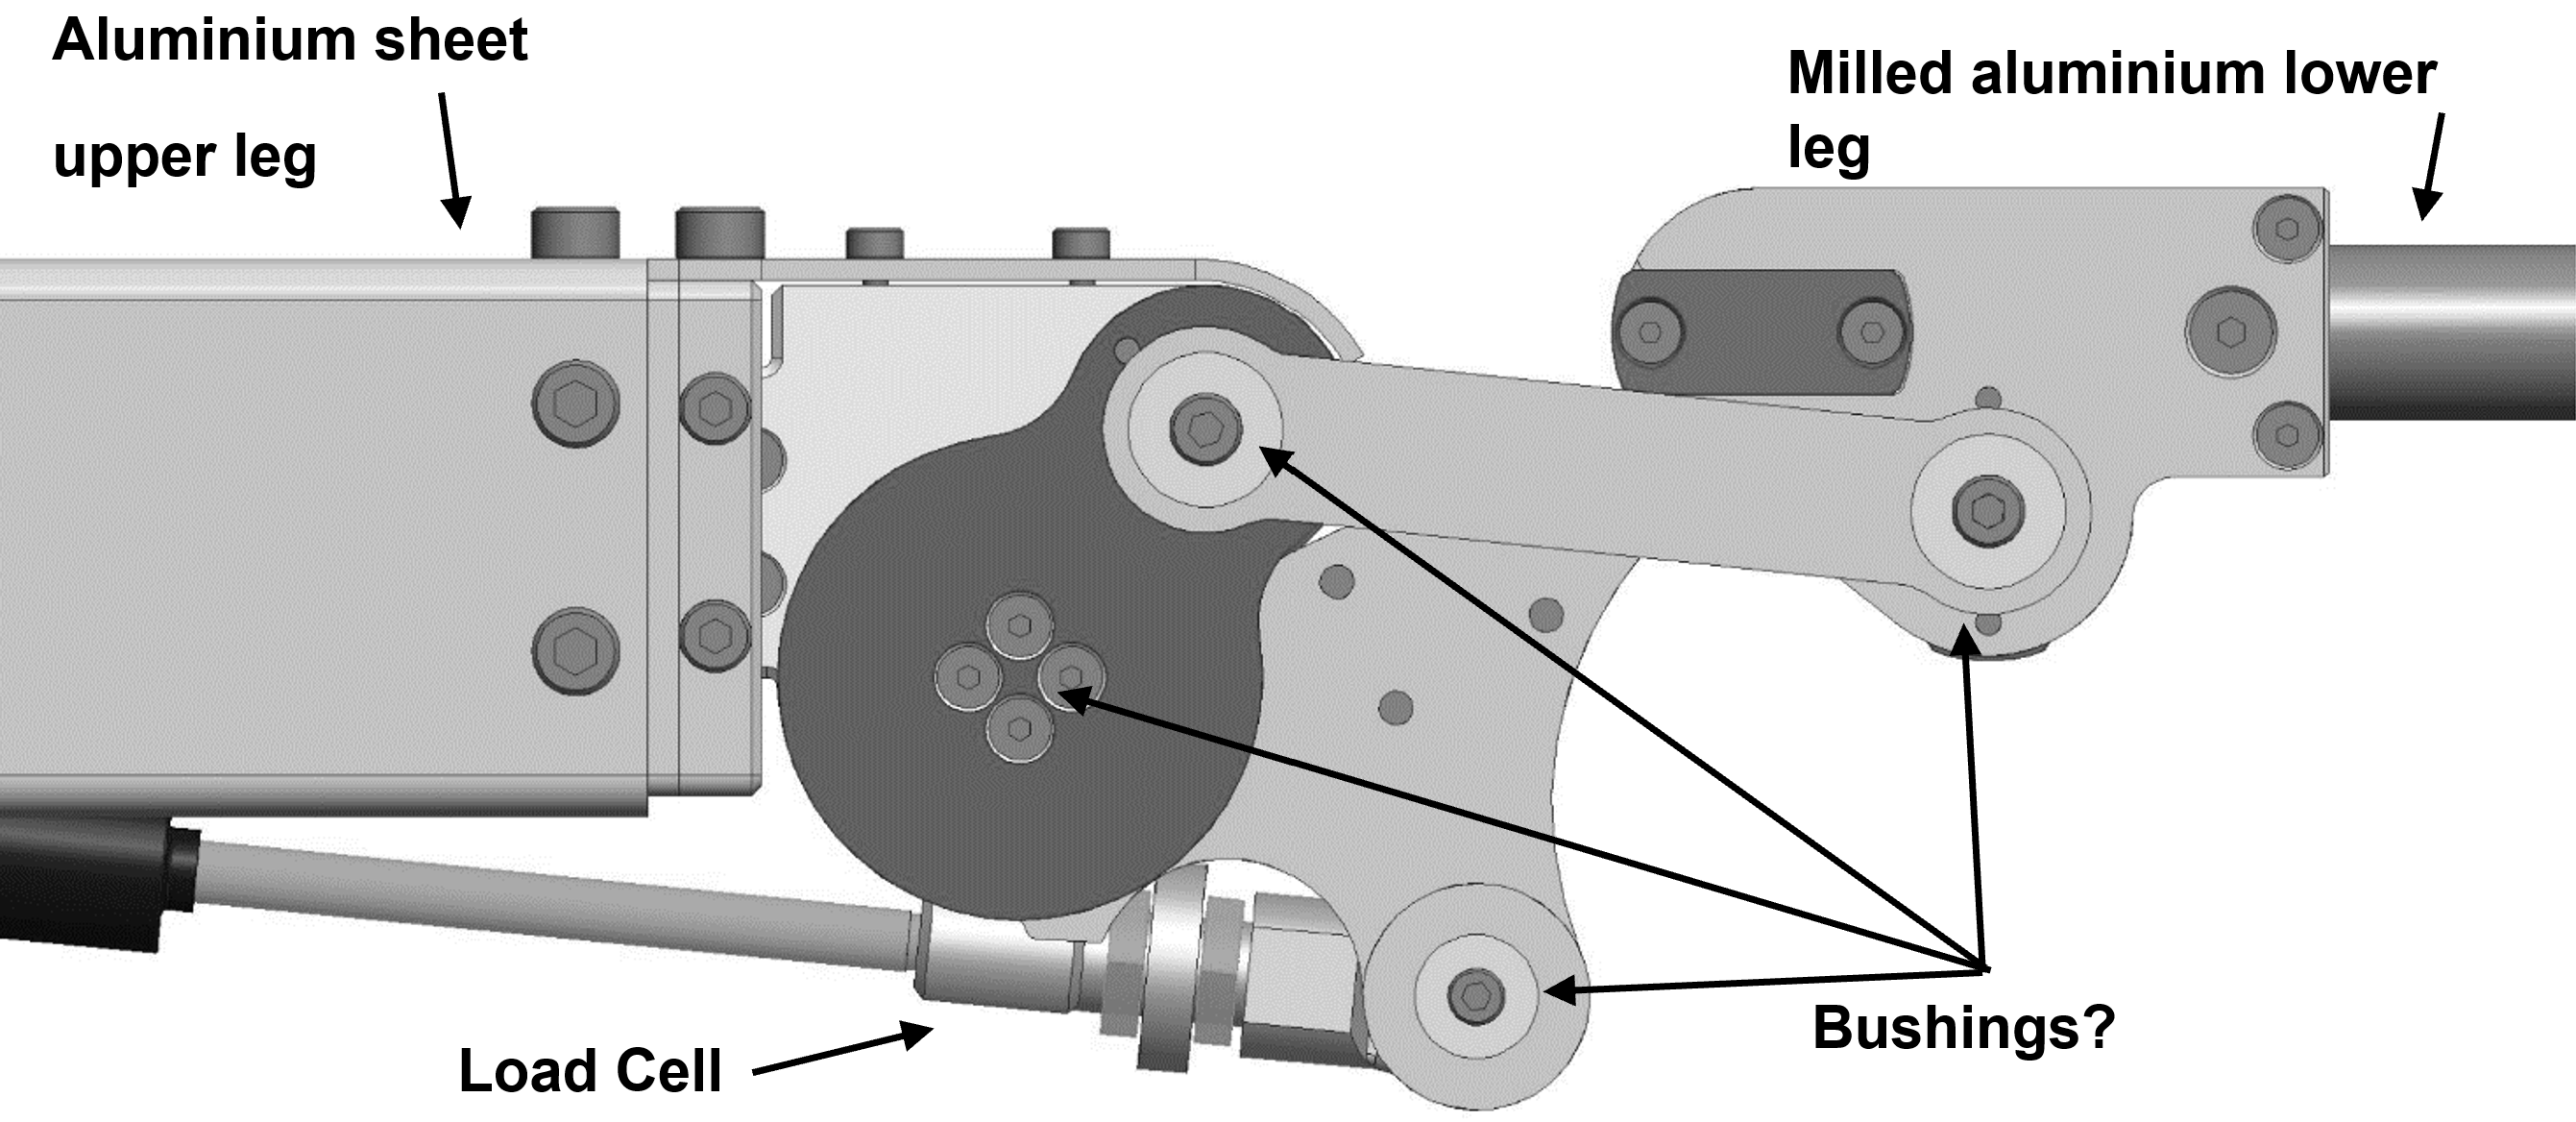
\includegraphics[width=0.7\textwidth]{Sections/LiteratureReview/img/minihyq/subsys_minihyq_knee_cad.png}
    \caption{MiniHyQ 4-bar linkage for knee joint \cite{khan_minihyq_2015}}
    \label{fig:minihyq_knee_cad}
\end{figure}

\begin{figure}[H]
    \centering
    \includegraphics[width=0.7\textwidth]{Sections/LiteratureReview/img/minihyq/subsys_minihyq_knee_links.png}
    \caption{MiniHyQ 4-bar linkage for knee joint kinematics \cite{khan_minihyq_2015}}
    \label{fig:minihyq_knee_links}
\end{figure}

\sssubsection{GOAT} \mbox{}\\

GOAT is an omni-directional leg morphology inspired by mountain goats \cite{kalouche_design_2016}.
Each leg contains 3  Tiger U10 brushless DC motors and single stage Matex 1:7 planetary gear stages, shown in Figure \ref{fig:goat_img}.
The author compared the performance of direct driven, quasi-direct driven, geared drive and series-elastic actuator driven actuators; the geared drive configuration for a single motor is shown in Figure \ref{fig:goat_motors}

\begin{figure}[H]
    \centering
    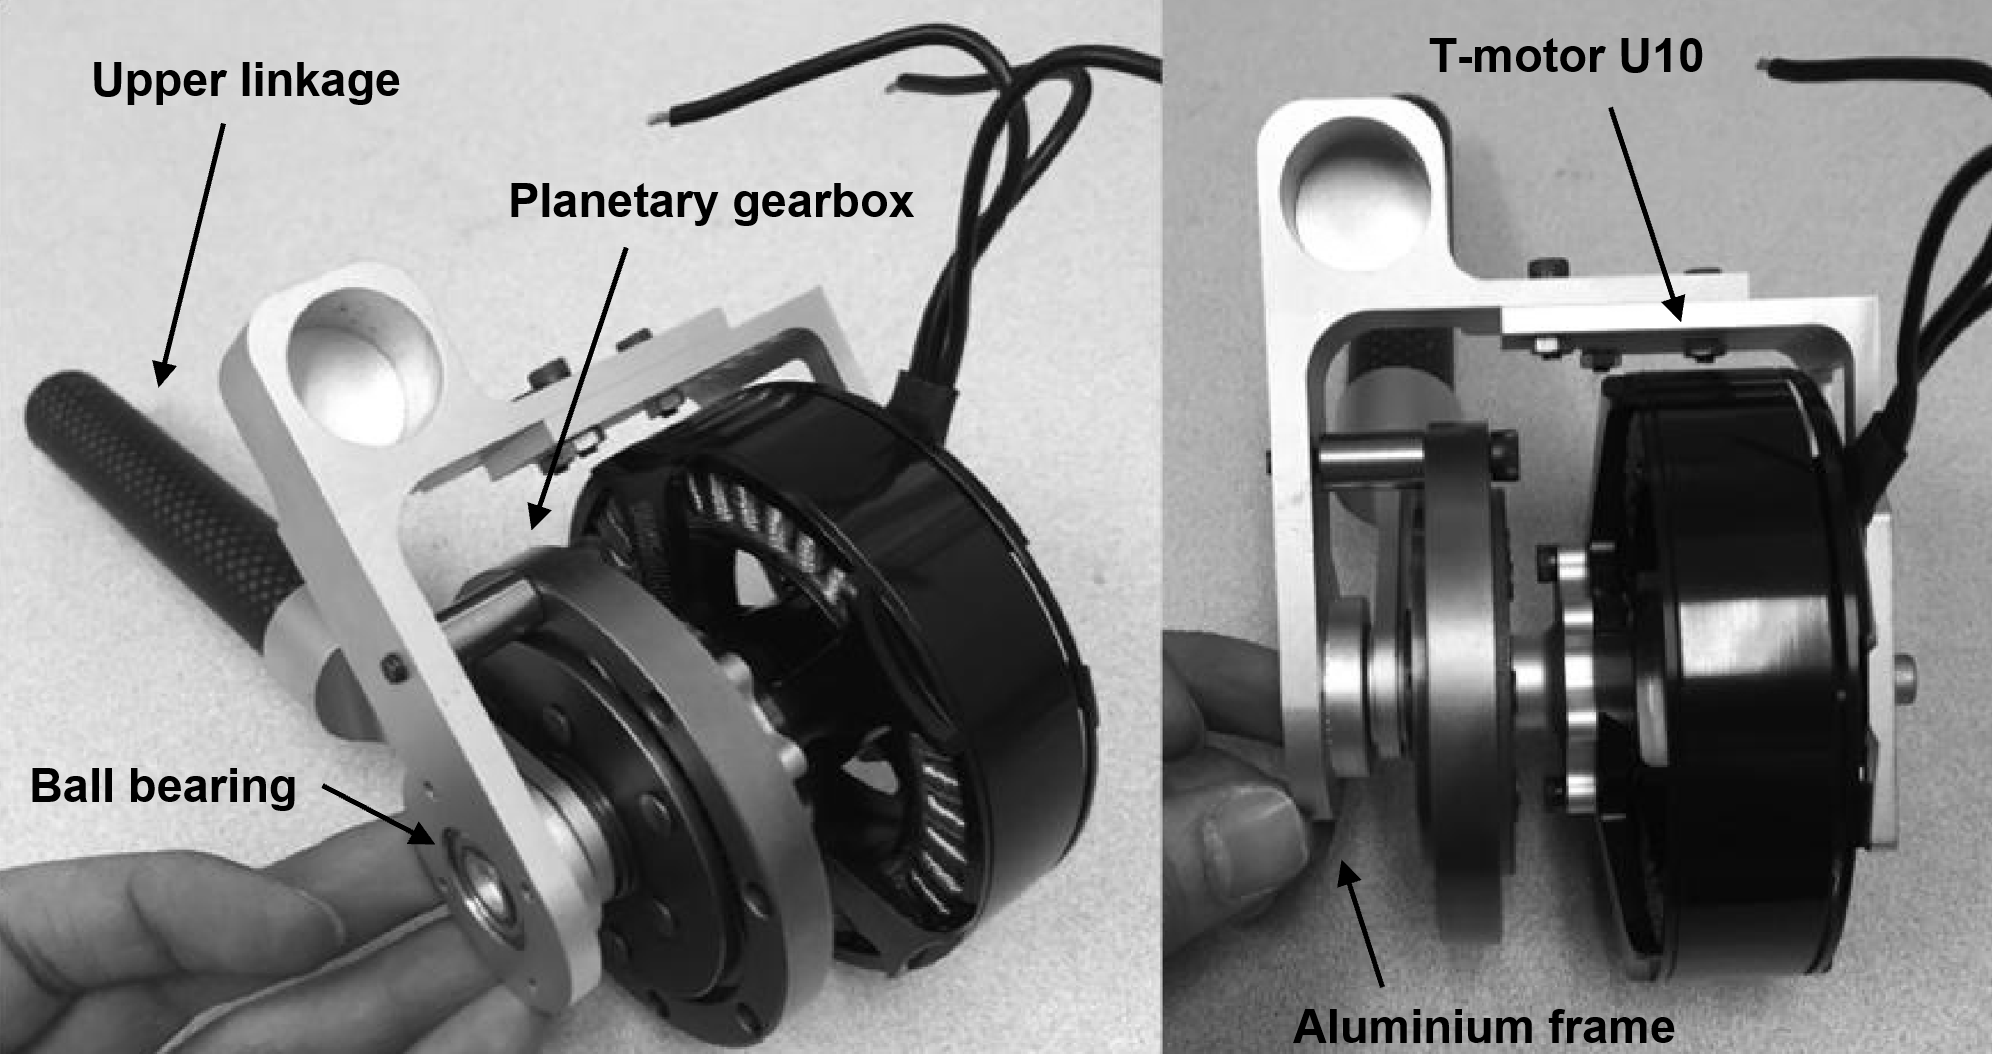
\includegraphics[width=0.8\textwidth]{Sections/LiteratureReview/img/goat/subsys_goat_motor.png}
    \caption{GOAT single motor and planetary gearbox \cite{kalouche_design_2016}}
    \label{fig:goat_motors}
\end{figure}

The knee joint shown in Figure \ref{fig:goat_knee} are composed of two ball bearings in the upper thigh, one needle bearing in the knee and two more ball bearings below the knee. The centers of rotation intersect to simulate a spherical joint.
This allows the GOAT knee to rotate with 3 DOF, but with a much greater range of motion for the compound joint ($90^{\circ}$ for the single needle bearing and $360^{\circ}$ for the other two sets of bearings), improving the work-space of the leg \cite{kalouche_design_2016}.
There is a singularity when the axes of the lower and upper leg align, removing a degree of freedom, however this is only achieved when the leg is virtual straight.
Carbon steel (1144) was used instead of aluminium for the bent knee piece as Von-Mises stresses exceeded aluminium's yield strength during hopping. Aluminium was used on the upper knee joint.
45558-HM Rockwest Composites carbon fibre rods are glued to the joints using Loctite Hysol E-120HP adhesive bonding.

\begin{figure}[H]
    \centering
    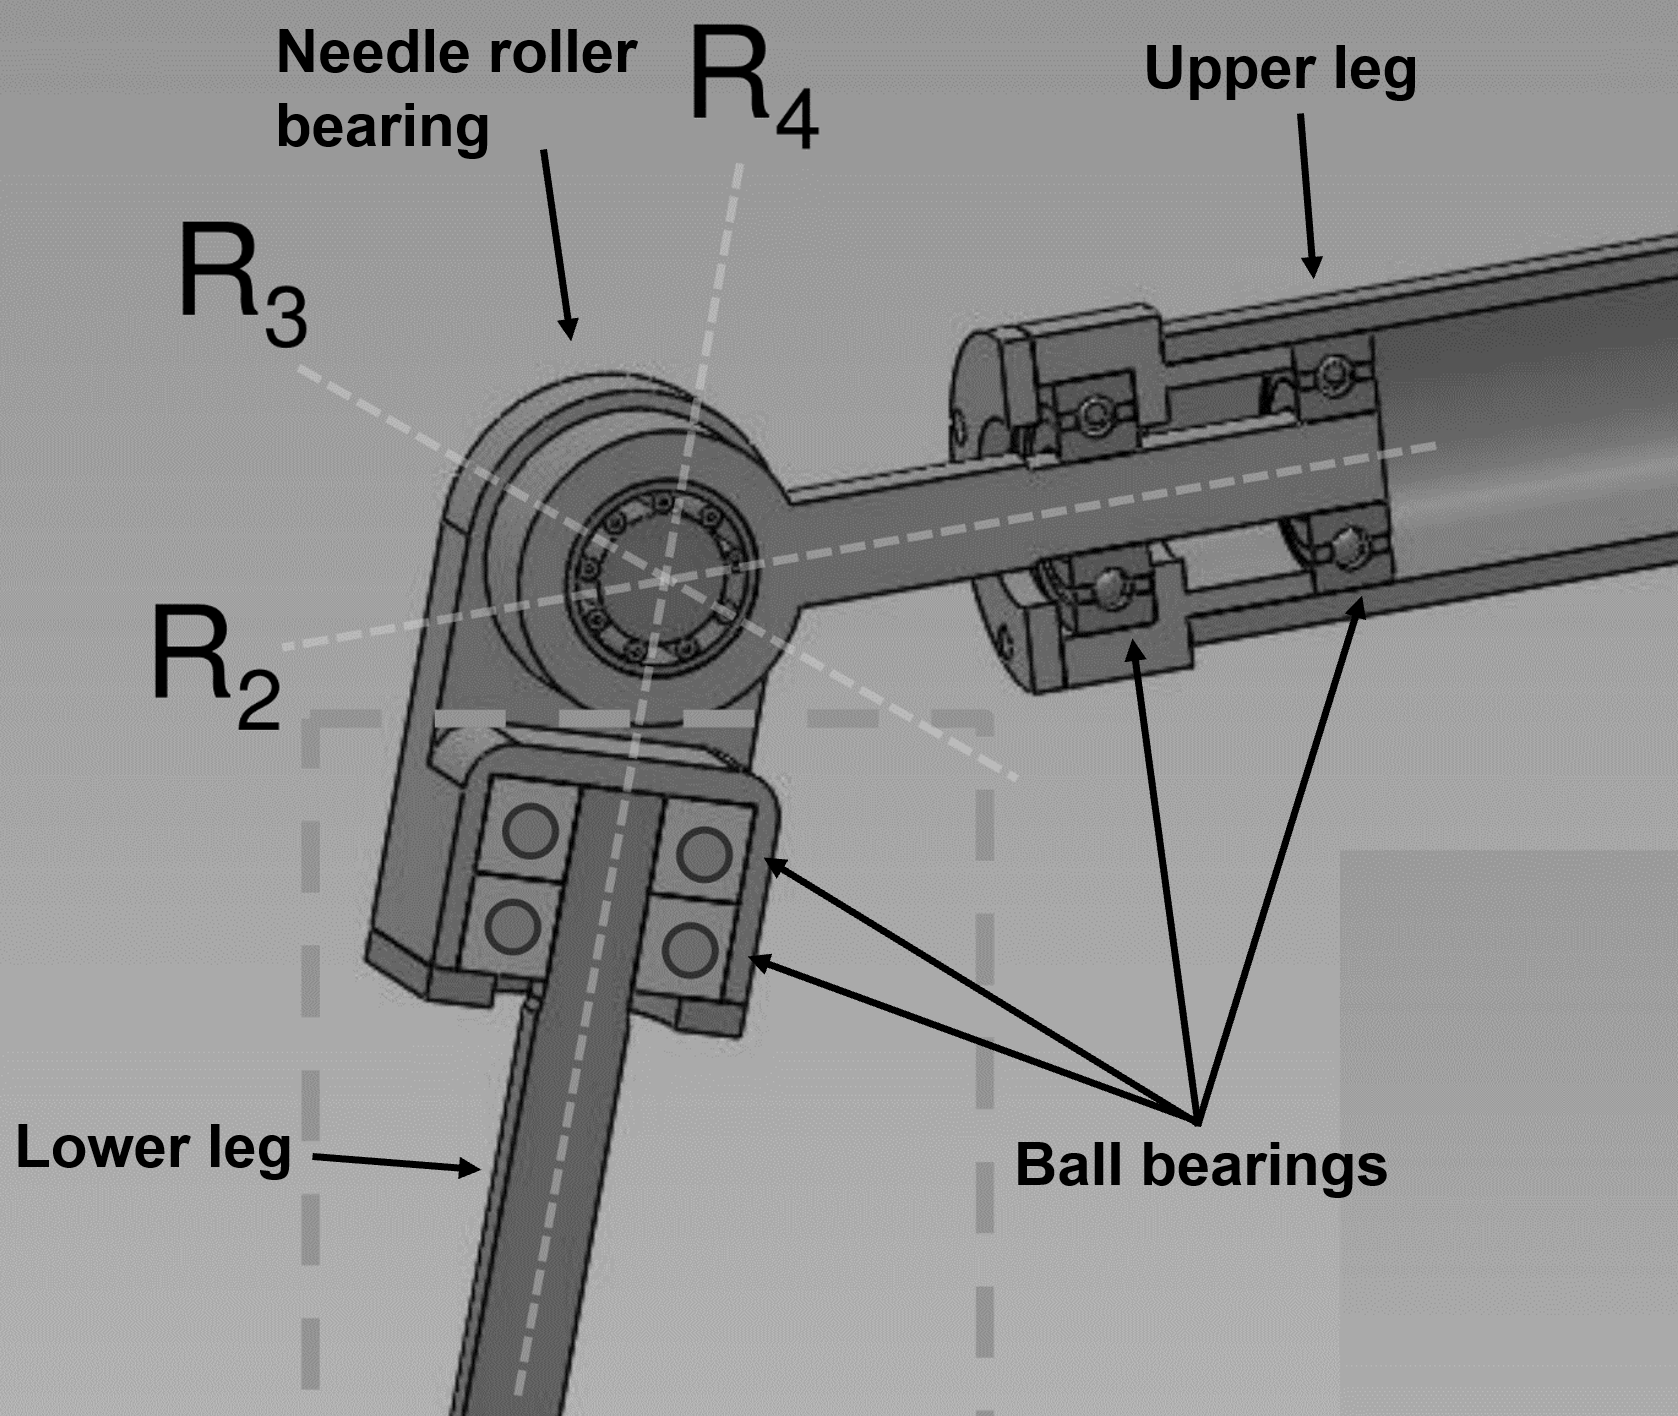
\includegraphics[width=0.6\textwidth]{Sections/LiteratureReview/img/goat/subsys_goat_knee.png}
    \caption{GOAT knee bearing configuration. Together, they mimic a spherical joint \cite{kalouche_design_2016}}
    \label{fig:goat_knee}
\end{figure}

\sssubsection{Stanford Doggo} \mbox{}\\
The legs of the Stanford Doggo are simple linkage mechanisms, providing 2 DOF. These consist of one axis of rotation at the hip, and the extension of the leg. There is no second axis of rotation at the hip, which makes it slightly more challenging for this robot to turn. However, this can be achieved through using different leg speeds for the right and left side legs, similar to a tank. They are powered by quasi-direct drive motors. This means that they use a lightweight belt drive instead of heavier planetary gears which are often employed in legged robots, such as the GOAT. This minimizes the inertia of the robot when attempting quick and high jumps, while also providing a high torque \cite{kau_stanford_2019}. The components of the leg system are shown in Figure \ref{fig:doggo_leg}. Two motors are used with belt drives to power coaxial drive shafts. These shafts each control the movement of one of the two upper leg linkages.

\begin{figure}[h]
    \centering
    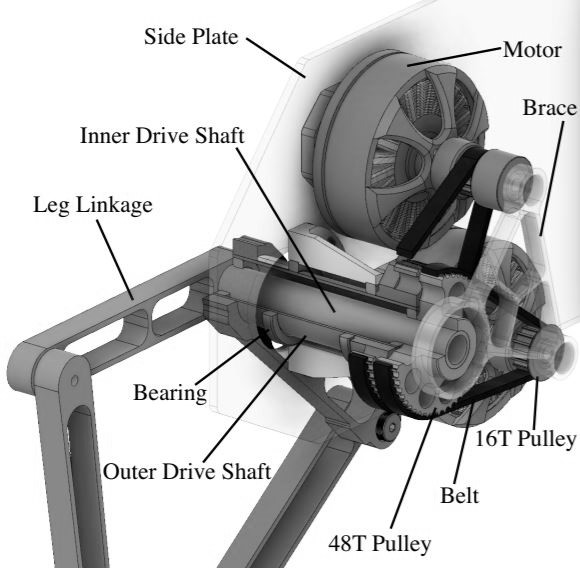
\includegraphics[width=0.55\textwidth]{Sections/LiteratureReview/img/doggo/subsys_doggo.JPG}
    \caption{Stanford Doggo leg and quasi-direct drive system components \cite{kau_stanford_2019}}
    \label{fig:doggo_leg}
\end{figure}

\sssubsection{CNC Hexapod} \mbox{}\\

The CNC Hexapod employs a fairly common topology allowing for 2 DOF around the hip and a single degree at the knee, all actuated by miniature servos and fastened using screws \cite{murshiduzzaman_hexapod_2019}.
The foot is attached to the leg via ball joint and uses gravity to retain its orientation.
The design is based on the Phoenix Hexapod of Lynxmotion, and trades aluminium links for perspex ones.
The hip configuration is very similar to the one found in Figure \ref{fig:multi-servo assembly}.
The leg is shown in Figure \ref{fig:cnchexapod_leg}.

\begin{figure}[h]
    \centering
    \includegraphics[width=0.7\textwidth]{Sections/LiteratureReview/img/cnchexopod/subsys_cnchexapod_leg.png}
    \caption{CNC hexapod leg morphology \cite{murshiduzzaman_hexapod_2019}}
    \label{fig:cnchexapod_leg}
\end{figure}

\sssubsection{Hexapod v2.1} \mbox{}\\

Each leg of the Hexapod v2.1 is driven by three independant servo motors to offer a total of 3 DOF per leg \cite{smallp_tsai_hexapod_2018}. The 3D printed links are first joined together using snap-fit connections and then secured using fasteners, as shown in Figure \ref{fig:hexapod_legass_img}. The output shaft of the servo motor is press fitted by hand onto the joint part. The opposite side joint is simply connected to the link with a small cylinder pin. The servo motors' housings only offer limited protection against harsh environments. This assembly has the advantage of being small, lightweight, and sufficiently sturdy for its application as a hobby or toy.

\begin{figure}[H]
    \centering
    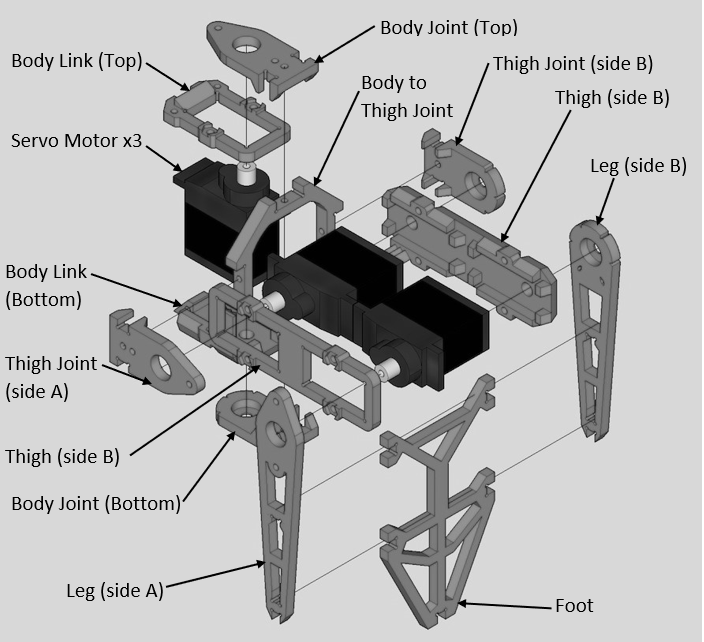
\includegraphics[width=0.7\textwidth]{Sections/LiteratureReview/img/hexapodV2.1/hexapod_v2p1_legass_ann.jpg}
    \caption{Hexapod v2.1 leg assembly components \cite{smallp_tsai_hexapod_2018}}
    \label{fig:hexapod_legass_img}
\end{figure}

\sssubsection{CRABSTER200} \mbox{}\\

The CR200 robot's locomotion is composed of four watertight dedicated legs and two arm-combined legs. The arm-combined legs have the same design as the dedicated legs with the addition of grippers to manipulate tools. As the leg assembly is complex, Figure \ref{fig:crabster_leg_dof_img} illustrates a simplified diagram of the joints' DOF for both types of legs. The hip yaw joint is mainly responsible for the forward propulsion of the hexapod. On the other hand, the hip roll joint and the knee roll joint are used to lift each leg from the ground to continue its gait. A 3 DOF leg, as used on the previous Hexapod v2.1, provides sufficient stability, but a fourth DOF within the hip pitch joint gives more flexibility to the CR200 for climbing and generating downward force when facing high tidal currents \cite{shim_development_2016}.

\begin{figure}[H]
    \centering
    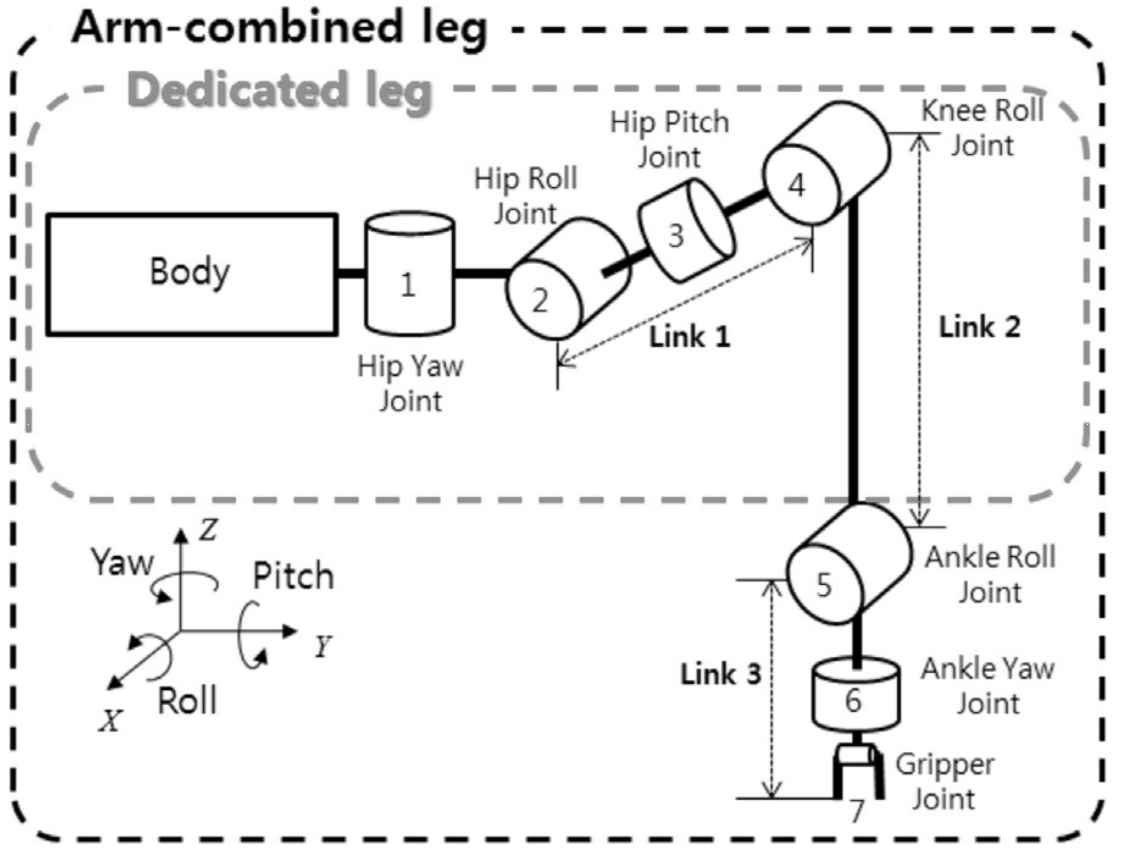
\includegraphics[width=0.8\textwidth]{Sections/LiteratureReview/img/Crabster/crabster_leg_dof.jpg}
    \caption{Dedicated and arm-combined leg joint schematic \cite{shim_development_2016}}
    \label{fig:crabster_leg_dof_img}
\end{figure}

Each dedicated leg joint is driven by a 640 W frameless BLDC motor that offers a maximum torque of 8.4 Nm \cite{shim_development_2016}. Each joint is also equipped with a harmonic drive gear set to transfer the reduced motion from the motor to the link, as shown on Figure \ref{fig:crabster_leg_joint_img}. Magnetic and optical incremental encoders are used to help control the motors while absolute encoders are used to track the angular position of each link. For the hip jaw joint, the input shaft is supported by a ball bearing on each side of the motor. The output shaft link is mounted on two ball bearings at the drive end of the link shaft and on a single ball bearing at the other end of the hip roll joint housing. In a similar way, the hip roll joint's input and output shafts are mounted on a single ball bearing on each side of the motor for a total of four bearings. Again, the idea remains the same for the hip pitch joint and the knee roll joint: both input and output shafts are mounted on two ball bearings distributed on each side of the motors, with the exception of the hip pitch joint's output shaft that has its two bearings on the external side between the input and output ends.

\begin{figure}[H]
    \centering
    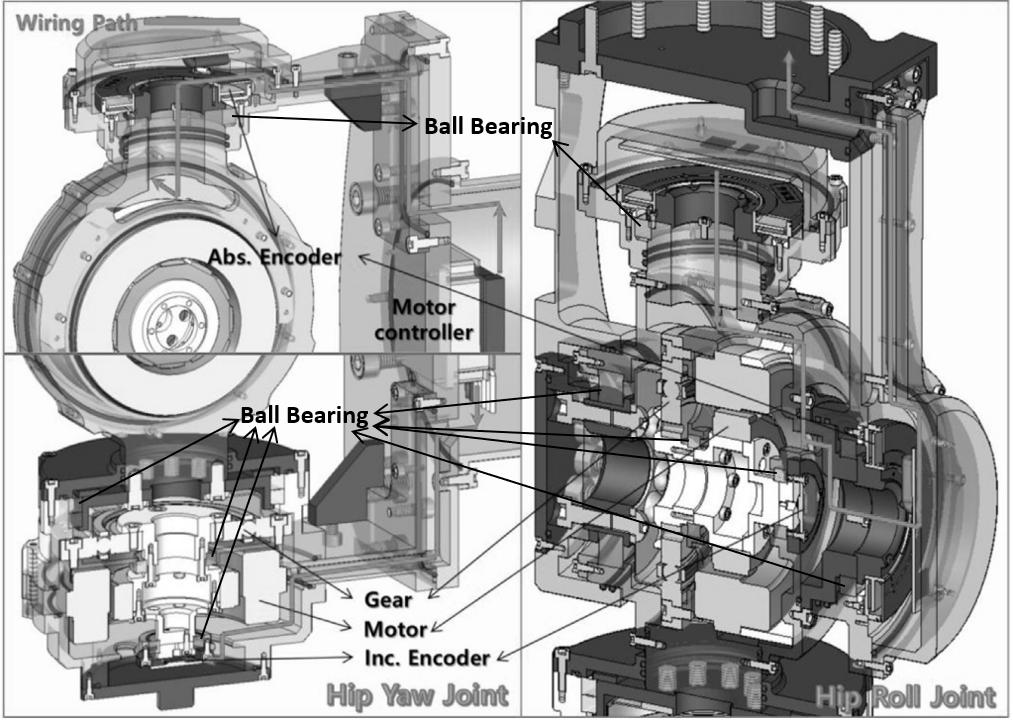
\includegraphics[width=\textwidth]{Sections/LiteratureReview/img/Crabster/crabster_leg_joint.jpg}
    \caption{Hip yaw and roll joint structure design (image best viewed in colour) \cite{shim_development_2016}}
    \label{fig:crabster_leg_joint_img}
\end{figure}

The watertight property is ensured with the use of single nitrile rubber type O-rings for flat contact surfaces and dual nitrile rubber type O-rings for cylindrical contact surfaces between two external housings as shown on Figure \ref{fig:crabster_watertight_img} \cite{shim_development_2016}. The pressure-resistant and watertight housings of the motors, reduction gears and sensors were tested in a hyperbaric test chamber with a pressure of 25 bar \cite{shim_development_2016}.

\begin{figure}[H]
    \centering
    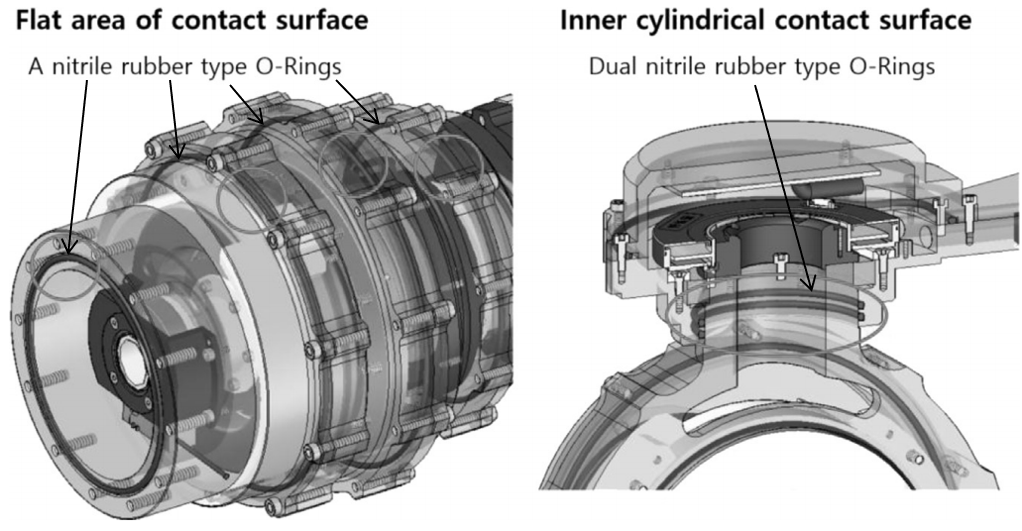
\includegraphics[width=\textwidth]{Sections/LiteratureReview/img/Crabster/crabster_watertight.jpg}
    \caption{The waterproof design with O-rings (image best viewed in colour) \cite{shim_development_2016}}
    \label{fig:crabster_watertight_img}
\end{figure}

%---------------------- FOOT ----------------------%

\subsubsection{Feet and Grip}

Most quadruped robots rely on high friction ball-shaped polymer feet.
GOAT, for example, has a half-sphere shaped foot coated in urethane rubber (see Figure \ref{fig:goat_img}).
As well as providing friction during motion, the coating also acts as a mechanical damper and filters out high frequency vibrations \cite{kalouche_design_2016}.
Stanford Doggo uses Dragon Skin silicone rubber to cover the cylindrical feet shown in Figure \ref{fig:doggo_leg} \cite{kau_nate711/stanforddoggoproject_2019}.
The CNC Hexapod leg shown in Figure \ref{fig:cnchexapod_leg} uses a flat foot and ball joint to keep it parallel to the ground \cite{murshiduzzaman_hexapod_2019}.
MiniHyQ does not specify how their foot functions, but from casual observation it too seems to simply be some solid rounded shape with rubber/polymer coating \cite{khan_minihyq_2015}. Similarly, CR200 does not specify the material used for the foot that makes contact with the ground. Each of its leg is equipped with a load cell with a thin cylinder plate that makes contact with the actual foot component \cite{shim_development_2016}. The leg from Figure \ref{fig:crabster_foot_img} seem to be covered by an aesthetically designed casing with a round tip to imitate the anatomy of the crab legs. Hexapod v2.1 does not rely on any particular foot shape which is most likely due to its negligible weight and its unique purpose of being a hobby robot.

\begin{figure}[h]
    \centering
    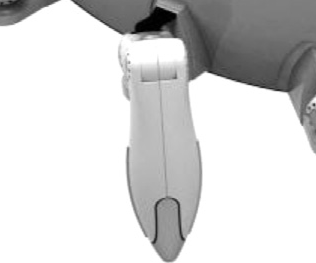
\includegraphics[width=0.4\textwidth]{Sections/LiteratureReview/img/Crabster/crabster_foot.png}
    \caption{Appearance of CR200's foot \cite{shim_development_2016}}
    \label{fig:crabster_foot_img}
\end{figure}

The challenge with a robot operating in rugged sandy or rocky beaches will be to ensure the feet do not dig into the ground excessively or get stuck. This could cause the robot to use more energy to move its legs due to the extra weight of the sand. A solution to this problem is applied in the use of snow shoes. These distribute weight on a larger area, thus decreasing the pressure applied on the snow surface, to limit how much a foot digs into snow \cite{edmonds_how_2009}. Snow shoe frames are also often made open, to limit accumulation of snow over-top. It is a similar method to the morphology of camel feet, which have developed to walk on desert sand. Their feet are composed of two closely located toes and are very soft, with thick leathery soles. This provides cushioning, as shown in Figure \ref{fig:foot_camel} which causes the feet to expand when stepped on, giving a larger surface area \cite{the_animal_facts_camel_nodate}.

\begin{figure}[H]
    \centering
    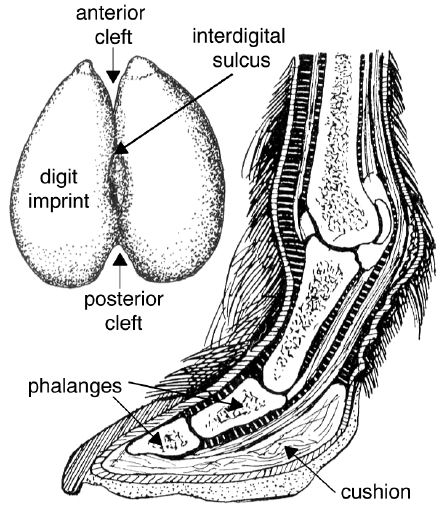
\includegraphics[width=0.4\textwidth]{Sections/LiteratureReview/img/Animals/foot_camel.JPG}
    \caption{The anatomy and print of a camel foot. \cite{lucas_ichnotaxonomy_2007}}
    \label{fig:foot_camel}
\end{figure}

%---------------------- CHASSIS ----------------------%

\subsubsection{Chassis}

Most existing quadruped and hexapod robots use aluminium sheets for their body (as found in MiniHyQ), or a combination of Aluminium sheets and Carbon Fibre sheets (as found in Doggo) \cite{khan_minihyq_2015} \cite{kau_stanford_2019}.
They are assembled using regular fasteners and standoffs for electronics. They are usually semi-open cases, which allow for optimal air-flow.
The Doggo chassis is shown in Figure \ref{fig:doggo_chassis}; standoffs, fasteners and electronics are visible.

\begin{figure}[h]
    \centering
    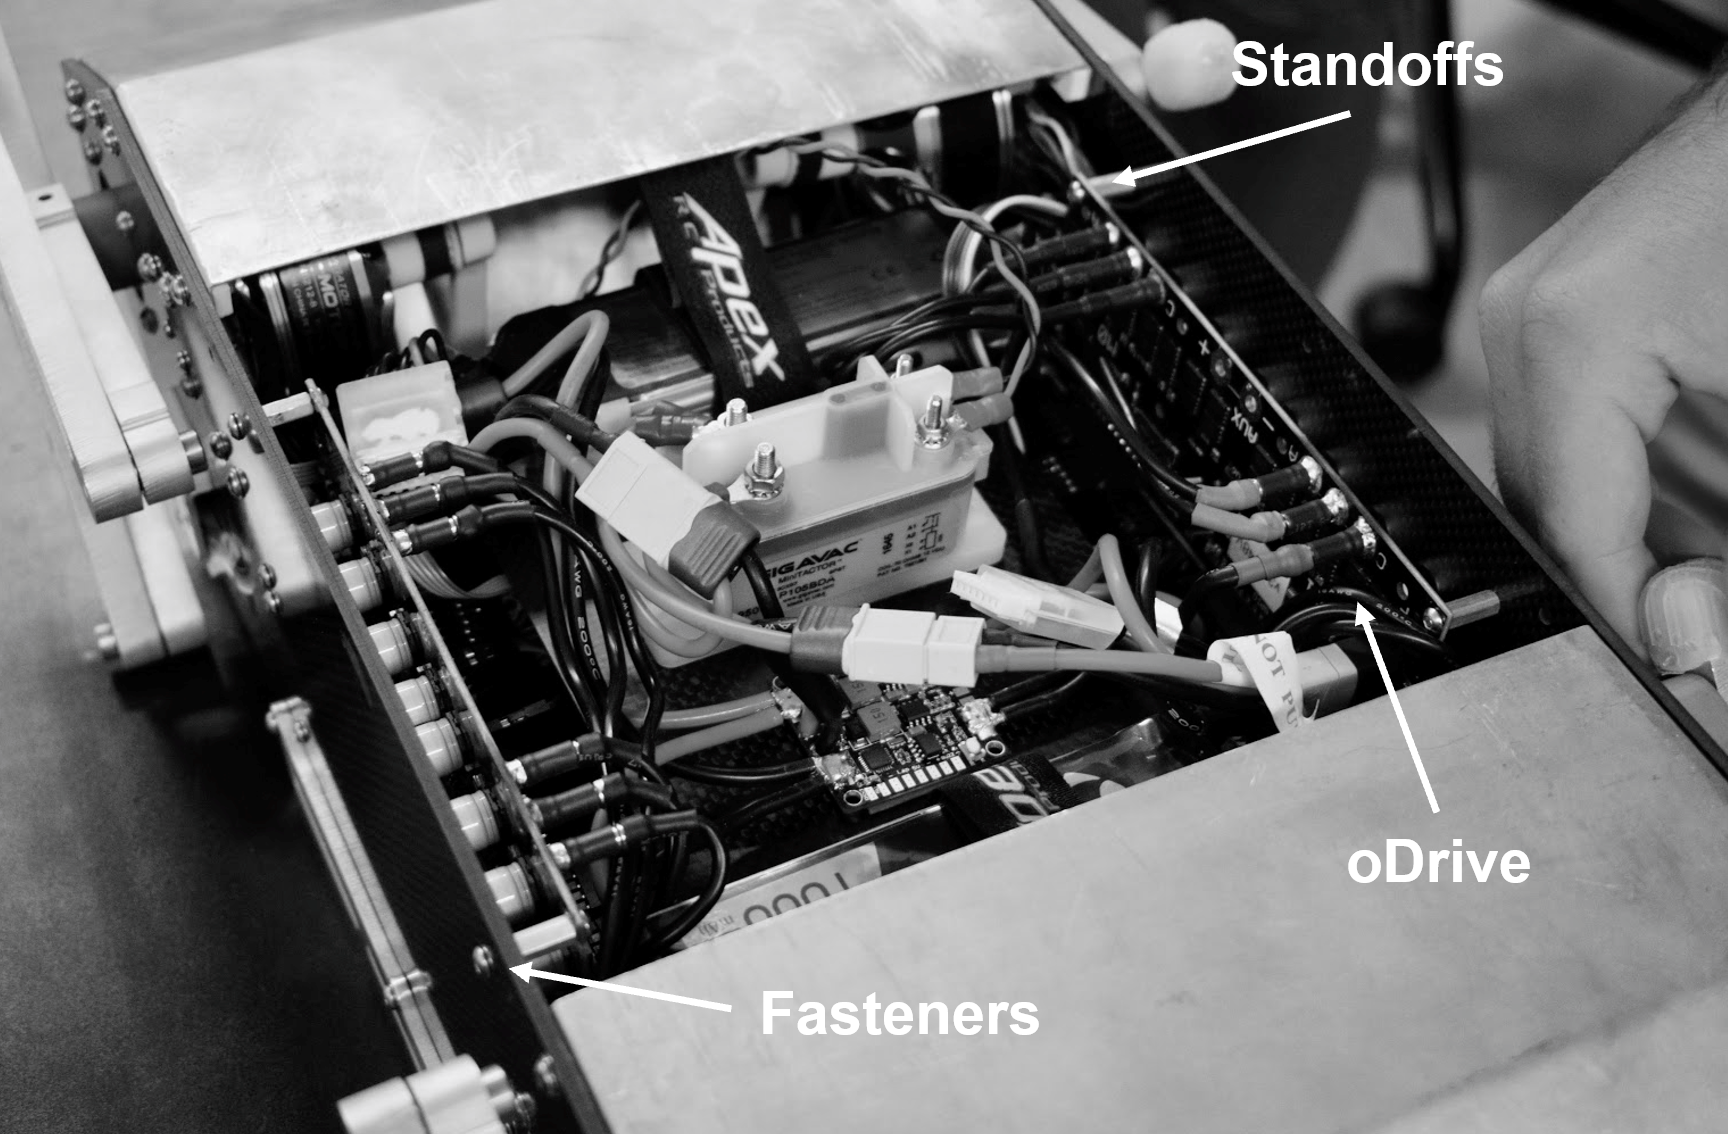
\includegraphics[width=0.7\textwidth]{Sections/LiteratureReview/img/doggo/subsys_doggo_chassis.png}
    \caption{Stanford Doggo chassis and components \cite{kau_stanford_2019}}
    \label{fig:doggo_chassis}
\end{figure}

Typical mounting of components to a robot chassis includes the use of bolts, washers, and nuts as shown in Figure \ref{fig:baisc_chassis_mounting} where two servo motors are mounted on a side plate. The same technique can be used for mounting power and computing equipment.

\begin{figure}[h]
    \centering
    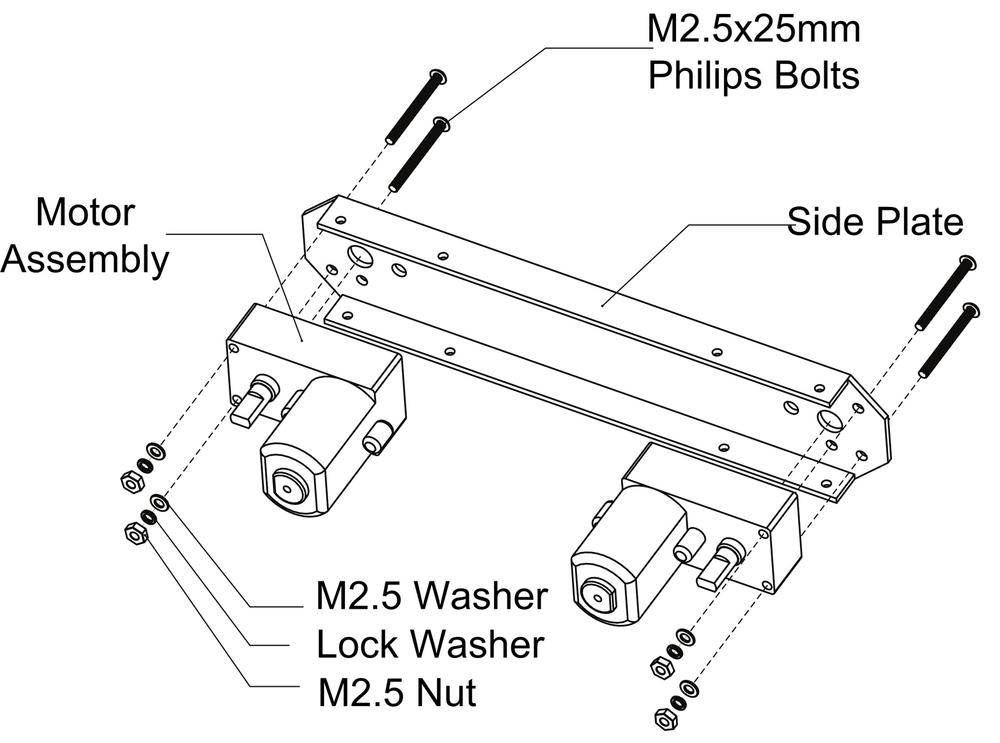
\includegraphics[width=0.6\textwidth]{Sections/LiteratureReview/img/Chasis/mountingBasic.jpg}
    \caption{Basic mounting procedure to a metal plate \cite{oreilly_building_nodate}}
    \label{fig:baisc_chassis_mounting}
\end{figure}


Additional plates and brackets can be mounted using standoffs and bolts as shown in Figure \ref{fig:extra_chassis_mounting}; in this figure an additional metal bracket is added for supplemental mounting capabilities. Furthermore, mounting brackets such as multi purpose brackets, servo brackets, U brackets, L brackets, C brackets, pan brackets, tilt brackets, plates, rails, angles, channels and custom designed brackets can use similar mounting procedures. 

\begin{figure}[h]
    \centering
    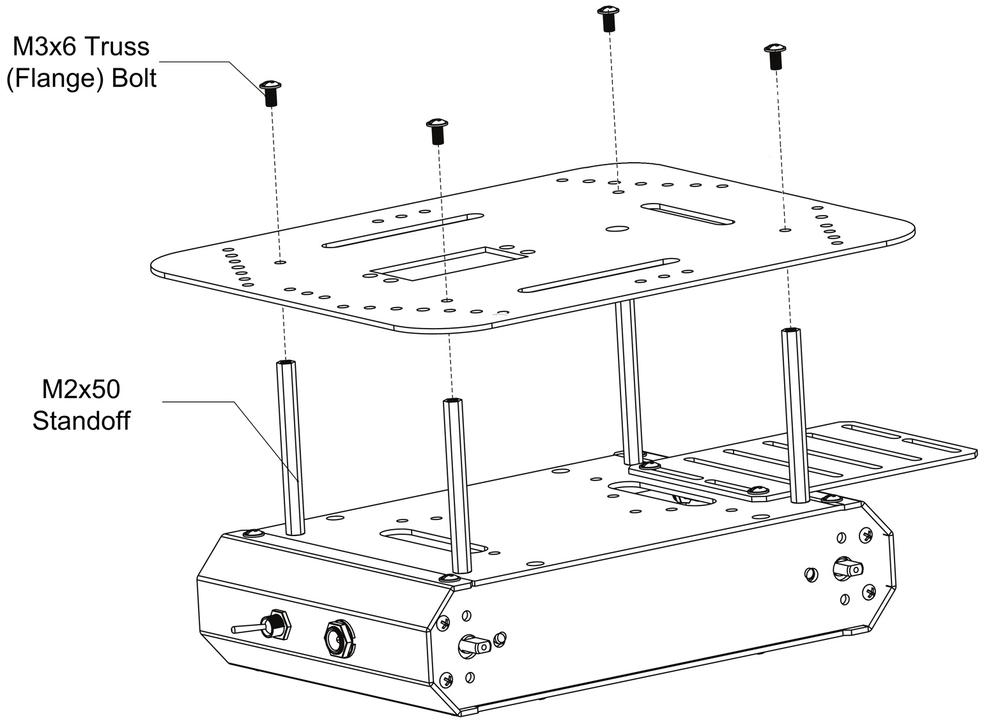
\includegraphics[width=0.6\textwidth]{Sections/LiteratureReview/img/Chasis/MountingExtraParts.jpg}
    \caption{Mounting of additional mounting plates \cite{oreilly_building_nodate}}
    \label{fig:extra_chassis_mounting}
\end{figure}

These designs, although simple, are insufficient for a waterfront environment, as they allow water, dust and other objects to enter.
The designs must thus be enhanced to meet weatherproofing standards.
IP67 gives complete protection against dust and contact, as well as immunity to water jets and immersion in 1 meter of water. Since the robot will operate on a beach and potentially in shallow water, this rating is appropriate \cite{dstm_ip_nodate}.
The equivalent NEMA rating, Type 6, can be achieved with the following enclosure considerations \cite{carey_how_nodate}:

\begin{itemize}
    \item Overlapping flanges on open seams
    \item Minimal number of seams
    \item Gaskets and O-rings at openings/joints
    \item Fasteners with included O-rings
    \item Even torque to screws for even O-ring/gasket compression
    \item Tight screw placement for even gasket pressure
\end{itemize}

An example of a waterproof hull and shell design mounted to interior plates, brackets and frame is shown in Figure \ref{fig:waterproof_shell}. This type of structure can be used to mount all electronic components on non water-resistant materials and conceal all equipment by mounting an exterior shell made of weatherproof materials and sealed to water, dust and sand particles.

\begin{figure}[H]
    \centering
    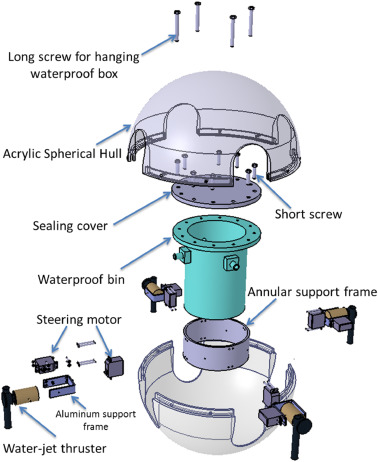
\includegraphics[width=0.6\textwidth]{Sections/LiteratureReview/img/Chasis/waterproofShell.jpg}
    \caption{Waterproof shell mounting \cite{guo_design_2017}}
    \label{fig:waterproof_shell}
\end{figure}

The CRABSTER200 shown in Figure \ref{fig:crabsterdetailed_img}, partially satisfies these watertight constraints. The mechanical components and housings of the CR200 hexapod are made of aluminium 6061 for easy fabrication while the chassis is made of a carbon fiber reinforced polymer (CFRP) composite and the shell skin is made of a glass fiber reinforced polymer (GFRP) composite \cite{shim_development_2016}\cite{yoo_design_2015}. In this case, the hull has an opening in the front for the too sled and therefore is not watertight, but the components within the body are well sealed with gaskets and O-rings \cite{shim_development_2016}.

%---------------------- POWER SYSTEMS ----------------------%

\subsubsection{Power System}

In order to be self-reliant and operate in remote areas, the waterfront robot must use a solar power system to generate the necessary power for its activities. A basic solar system consists of photovoltaic solar cells generating DC power which is fed through a regulator. This regulator ensures that the batteries do not get damaged. In the case where AC power is required, an inverter is used \cite{solar_power_australia_solar_nodate}. These components are shown in Figure \ref{fig:power_system}.

\begin{figure}[H]
    \centering
    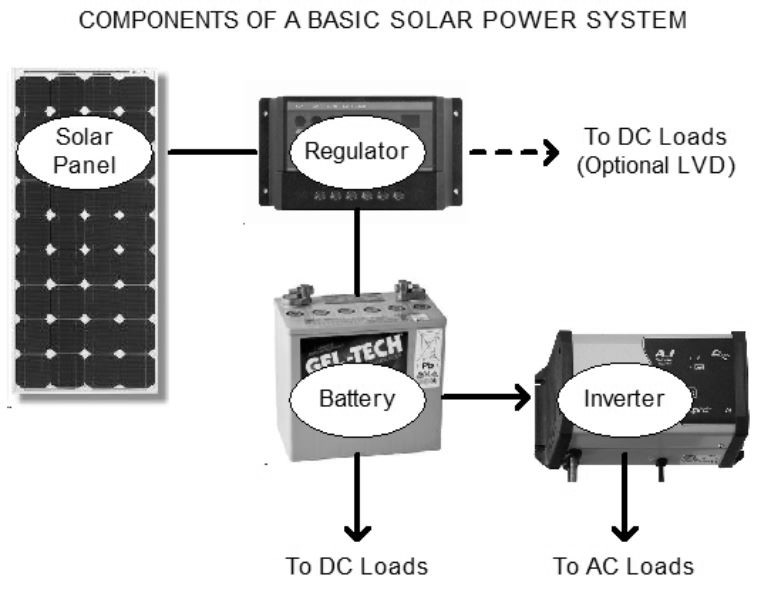
\includegraphics[width=0.6\textwidth]{Sections/LiteratureReview/img/solar/power_system.JPG}
    \caption{Solar panel system components \cite{solar_power_australia_solar_nodate}}
    \label{fig:power_system}
\end{figure}

To give an approximate idea of the specifications of solar panels, suggested off-grid RV solar panels were found by Wholesale Solar. A 100 W rigid solar panel (SLP100-12U) weighs 8.9 kg and has a surface area of 0.72 m$^{2}$. It is composed of 36 solar cells \cite{wholesale_solar_solarland_nodate}. Technical specifications are provided in the Appendix \ref{app:solar}. The panel's weight is considerable for a robot to hold, and is almost twice the weight of the Stanford Doggo \cite{kau_stanford_2019} mentioned previously. Considering this robot can operate at 840 W, one 100 W panel may also not be sufficient to maintain a reasonable operation time or speed. The energy collected by the solar panels would be stored in the battery which would allow the robot to work. However once the battery is depleted, the solar panel alone would not be sufficient. The robot might thus require to take battery charging breaks during the day. Rigid solar panels can be mounted to a surface using a rack with clamps. An example of an assembly is shown in Figure \ref{fig:solar_rack1} \cite{gogreensolar_ironridge_2015}.

\begin{figure}[H]
    \centering
    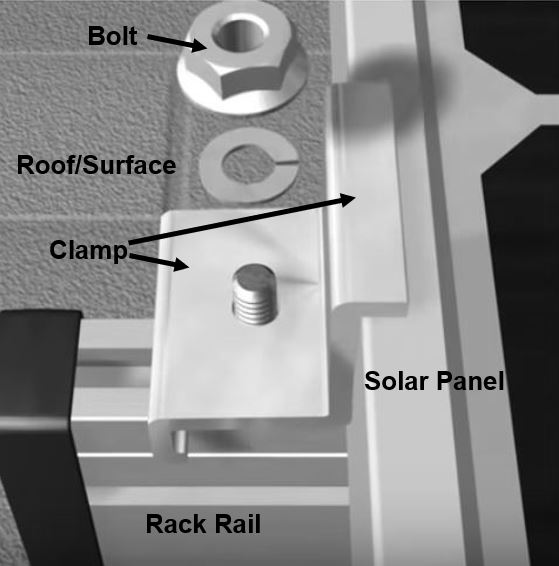
\includegraphics[width=0.5\textwidth]{Sections/LiteratureReview/img/solar/solar_rack1.JPG}
    \caption{Rack mounting system for rigid solar panels \cite{gogreensolar_ironridge_2015}}
    \label{fig:solar_rack1}
\end{figure}

Another option would be to use flexible solar panels. A 100 W model (SPR-E-Flex-110) recommended by Wholesale Solar for RV's (comparable to the previous rigid solar panel shown) weighs only 2 kg and has a surface area of 0.64 m$^{2}$. It contains 32 solar cells \cite{wholesale_solar_sunpower_nodate}. The small weight of the flexible solar panel compared to the rigid type could contribute to a better efficiency of the robot system, as a small weight takes less energy to move around. Technical specifications are provided in the Appendix \ref{app:solar}. This type of solar panel can be bent up to 30 degrees and is better adapted to rugged environments \cite{powerscout_should_2017}. They are easily mounted flush onto a flat or curved surface using adhesives or grommets integrated onto the sides of the panel \cite{wholesale_solar_sunpower_nodate}. Figure \ref{fig:solar_bolt} shows how to use a bolt kit to mount the flexible panel on canvas \cite{custom_marine_products_flexible_nodate}. This method could be used for other thin mounting surfaces as well.

\begin{figure}[H]
    \centering
    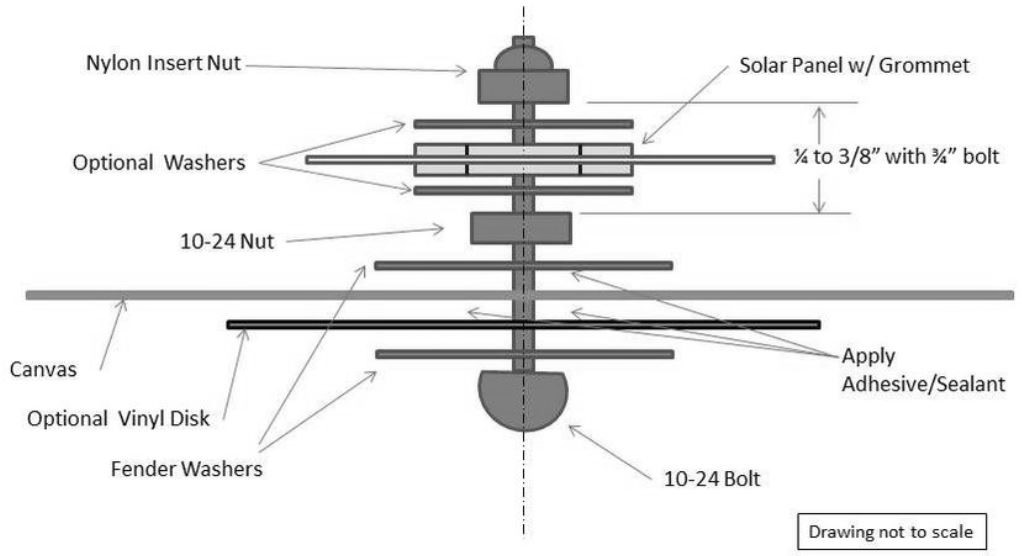
\includegraphics[width=0.8\textwidth]{Sections/LiteratureReview/img/solar/solar_bolt.JPG}
    \caption{Bolt mounting for flexible solar panels onto canvas (or other thin materials) \cite{custom_marine_products_flexible_nodate}}
    \label{fig:solar_bolt}
\end{figure}

Due to the mobile and rugged nature of the application, a more custom solar system solution may be required. It is possible to obtain custom solar panels from many providers such as Voltaic Systems \cite{voltaic_systems_custom_nodate} and Hovall \cite{hovall_custom_nodate}. The required dimensions, shapes, connections, specifications and more can be accommodated. It is also possible to obtain solar cells on their own (not made into a panel). A very efficient flexible solar cell, the MAXEON, is available from Sunpower. These cells each weigh 6.5 g and have dimensions of 125 X 125 mm. Their peak power output is of about 3.54 W \cite{sunpower_buy_2017}. More details are provided in Appendix \ref{app:solar}. Tabs weighing 0.3 g each are used to attach the solar cells together (these are mentioned in the solar cell specifications in the appendices). By comparing the area of the previously mentioned flexible solar panel (recommended by Wholesale Solar \cite{wholesale_solar_sunpower_nodate}) with the equivalent area in these solar cells (while also taking into account space for connecting tabs), it is estimated that they would provide about 125 W in power, instead of only 100 W.

As mentioned previously, a solar regulator is required to regulate the power going to the battery.
It is chosen based on the amount of amperage that it can accept from solar panels. Thus, it should be able to accommodate the sum of the maximum current of all the solar panels in the system. It is also best to increase this number, as in ideal conditions, a solar panel could produce slightly more energy than specified \cite{smith_caravansplus:_nodate}. Both the previously mentioned panels (rigid and flexible panels) have a maximum current of about 6 A \cite{wholesale_solar_sunpower_nodate} \cite{wholesale_solar_solarland_nodate}. Assuming that the robot might require two or more 100 W solar panels, a 20 A regulator (SRP0240) was found from REDARC Electronics. It weighs only 0.26 kg and has dimensions of 153 x 76 x 37 mm \cite{redarc_electronics_20a_nodate}. Additional specifications are shown in Appendix \ref{app:solar}. It can be easily mounted on a surface using fasteners, as shown in Figure \ref{fig:solar_reg}.

\begin{figure}[H]
    \centering
    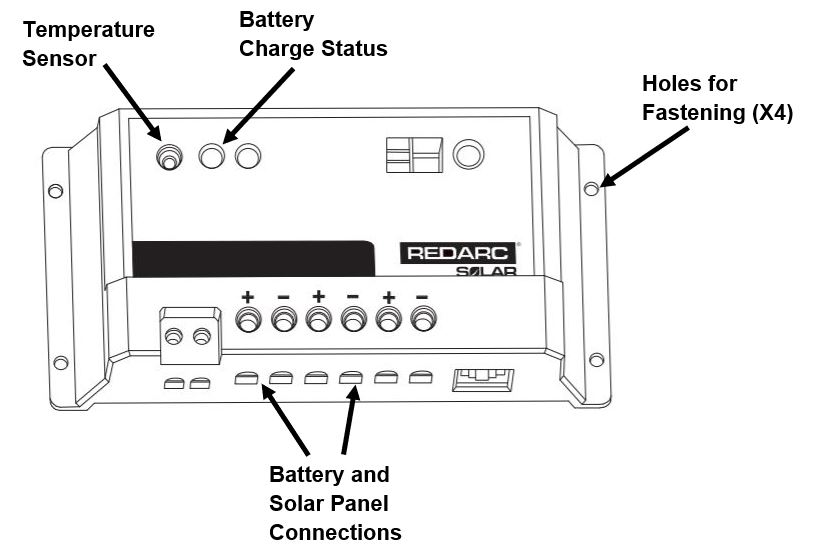
\includegraphics[width=0.7\textwidth]{Sections/LiteratureReview/img/solar/solar_reg.JPG}
    \caption{Configuration and mounting of a regulator by REDARC Electronics \cite{redarc_electronics_20a_nodate}}
    \label{fig:solar_reg}
\end{figure}

%---------------------- DRIVE SYSTEM ----------------------%

\subsubsection{Drive System: Motors and Gear Reducers}

Electrical motors are separated into two main categories: AC and DC motors, with DC separated into brushed and brushless motors. The differences between an AC and DC motor, apart from their input current type, is the efficiency, service life, and operation.

As DC motors use permanent magnets, less energy is lost in the creation of electromagnets and will provide flat torque over wider speed ranges compared to AC motors \cite{oriental_motor_brushless_nodate}. However, AC motors tend to have higher life expectancy than DC motors \cite{ohio_electric_motors_what_2015}. Brushless DC motor will have a higher efficiency compared to brushed DC motors due to the absence of friction \cite{oriental_motor_brushless_nodate}\cite{robots_shop_24v_nodate}. 
See specifications sheet in appendices.
Common DC motor manufacturers include Maxon Motor and T-motor; the former develops stepper motors designed for industry and robotics \cite{maxon_motor_applications_nodate}. Their power consumption is between a Watt and 500W, output torques up to 1 Nm without gearing, and diameters between 6 and 90mm \cite{maxon_motor_maxon_nodate}.
T-motor develops DC motors for multirotor and fixed wing aircrafts \cite{t-motor_t-motor_nodate}.
Stanford Doggo and Simon Kalouche's GOAT both use T-MOTORS to actuate their legs, along with belt drives and planetary gearboxes \cite{kalouche_design_2016} \cite{kau_nate711/stanforddoggoproject_2019}.
Their motors scale from a few watts to 10 000W for their largest unit.
Because they are not stepper motors, a special motor driver is required to manipulate them to precise positions; in the case of GOAT, it is custom made, whereas Stanford Doggo leverages oDrives \cite{weigl_odrive_nodate}.


To operate at a motor's most efficient or nominal point, the output speed of the motor should be maximized and output torque minimized \cite{khan_minihyq_2015}. To achieve this, gear reducers are mounted on the output shaft to achieve a more usable speed (RPM) and torque level. Different types of gear reducers exist, such as planetary; parallel and right angle shaft; and worm gears \cite{groschopp_motor_2018}. Small planetary gears with 100:1 ratios are available for rated speeds between 3000 RPM and 5000 RPM. They are priced at  70 to 200 CAD depending on the size of the shaft or NEMA type \cite{banggood_nema_nodate}. Even smaller gears can be found with reduced ratios when applicable; for example, the Matex 7:1 planetary gearbox used by GOAT weighs 0.2 with a 7:1 ratio kg\cite{kalouche_design_2016}. Matex's smallest metal offering has a 3:1 ratio, measures 25mm in diameter, 13mm in depth and weighs 20g \cite{matex_sintered_nodate}. Gear boxes are mounted using the designated mounting holes, and a shaft coupling mechanism. As shown in Figure \ref{fig:gear_box}, the gear reducer is mounted using 4 screws and bolts, and the shaft coupling uses a keyway.

\begin{figure}[H]
    \centering
    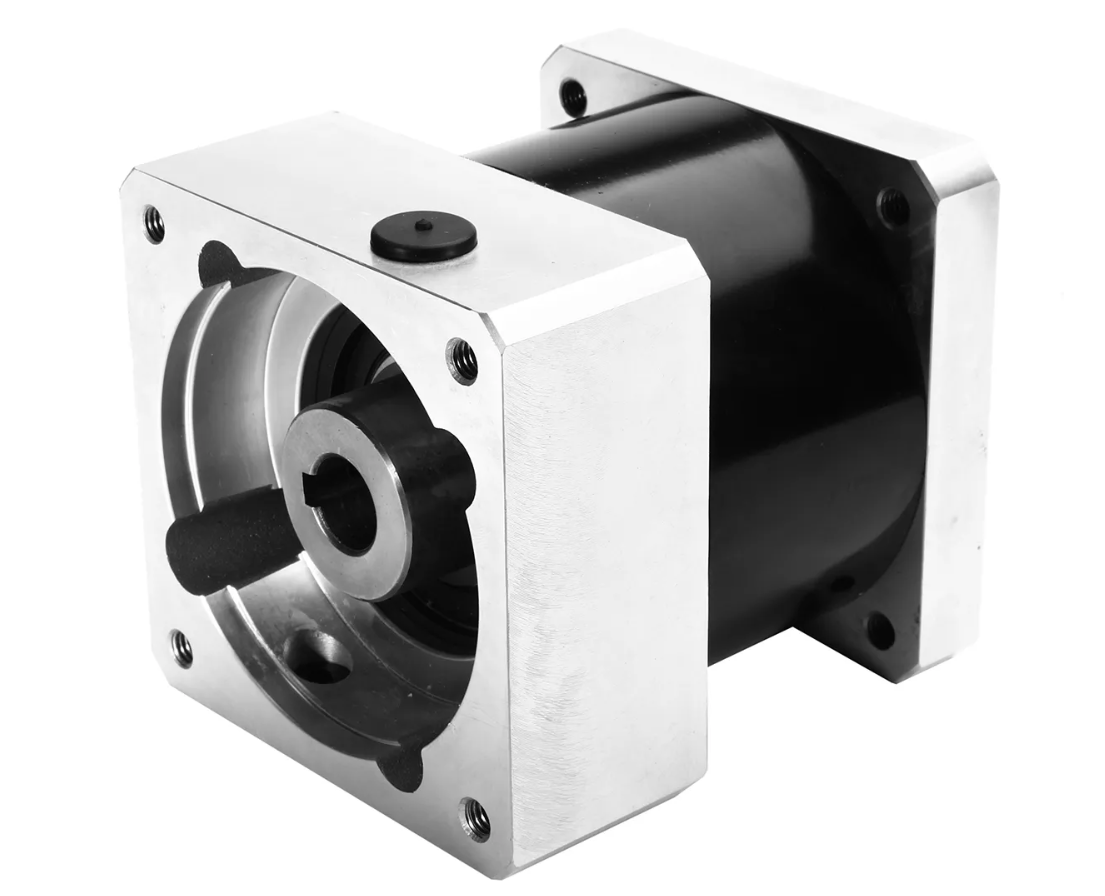
\includegraphics[width=0.5\textwidth]{Sections/LiteratureReview/img/drive/GearBox.PNG}
    \caption{Planetary gear box with mounting points \cite{banggood_nema_nodate}}
    \label{fig:gear_box}
\end{figure}

%------------------------ MOTORS ------------------------%
\sssubsection{Gear Motors} \mbox{}\\

Gear motors are a combination of motor and gear reducer. They vary in shapes, sizes, weight, power, and speed. 

The type and direction of the output shaft can vary. As shown in Figure \ref{fig:output_shaft_gear_motor} the output shaft can be parallel or perpendicular to the motor, and the shaft can be hollow or solid. 

\begin{figure}[H]
    \centering
    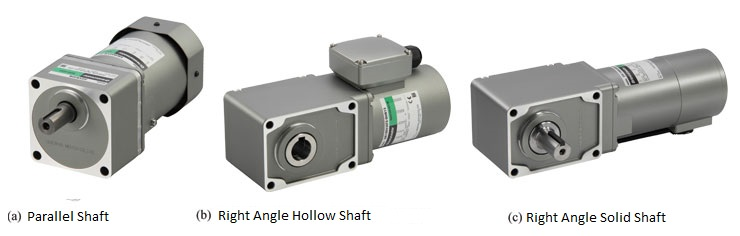
\includegraphics[width=1\textwidth]{Sections/LiteratureReview/img/LegAssembly/OutputTypeGearMotor.jpg}
    \caption{Output Shaft types and configurations. \cite{essence_automation_products_2018}}
    \label{fig:output_shaft_gear_motor}
\end{figure}

Gear motors come with multiple mounting configuration types. Figure \ref{fig:foot_mounting _frame} illustrates two configurations: flange mounting and foot mounting. 

\begin{figure}[H]
    \centering
    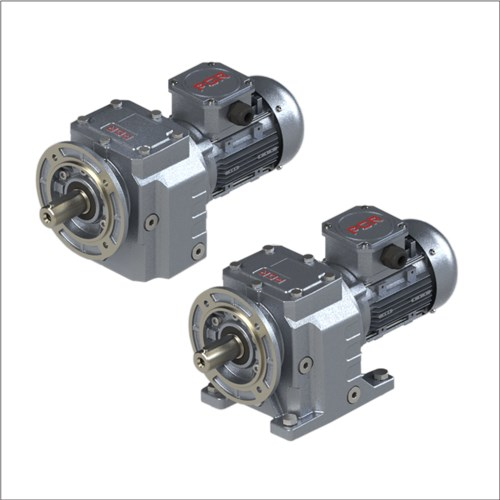
\includegraphics[width=0.5\textwidth]{Sections/LiteratureReview/img/LegAssembly/flange_foot_mounted_gearMotor.jpg}
    \caption{Flange (Left) vs. Foot (Right) Gear Motor Frame Mounting. \cite{dinamik_motor_foot-flange_nodate}}
    \label{fig:foot_mounting _frame}
\end{figure}

The Figure \ref{fig:form_mounting} illustrate how the foot mounting configuration can be used to position the gear motor in multiple different configurations. 

\begin{figure}[H]
    \centering
    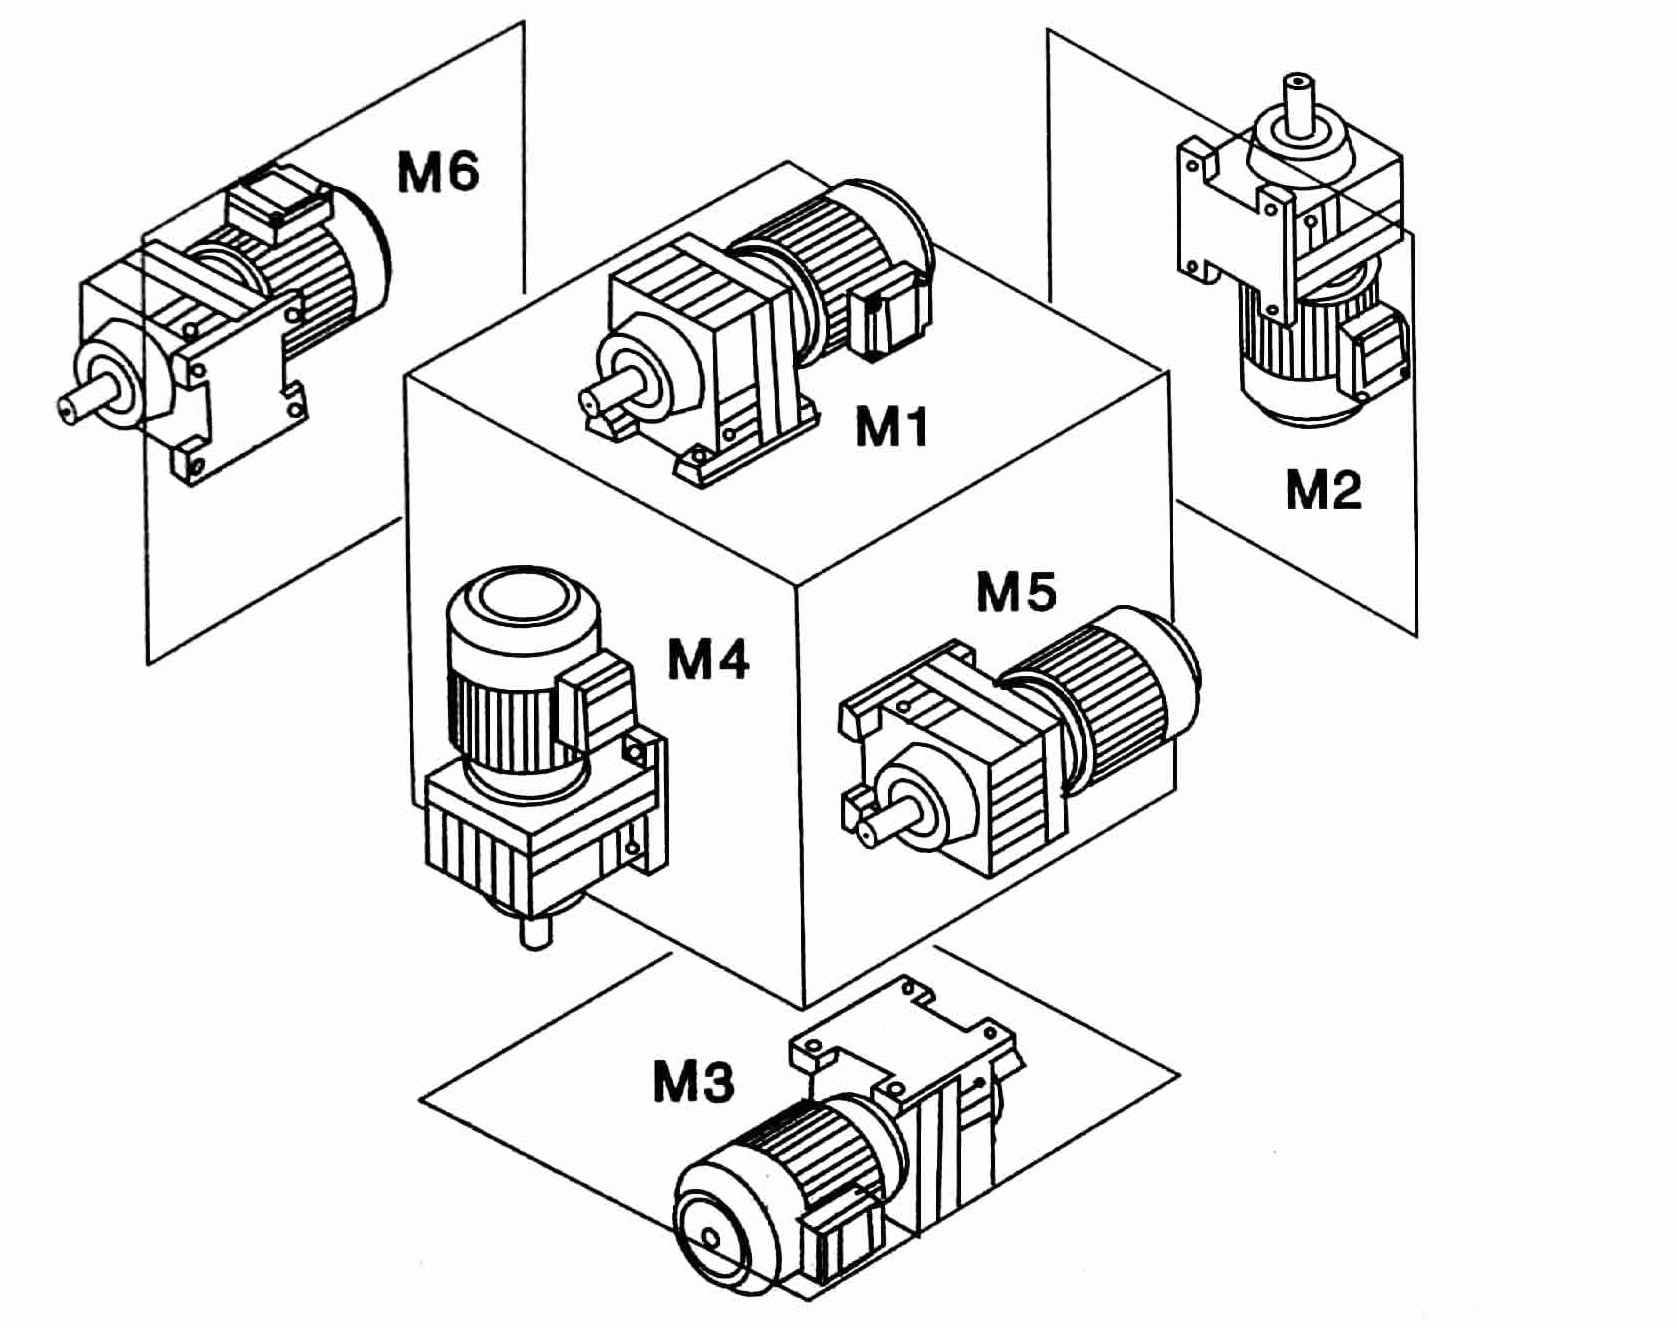
\includegraphics[width=0.5\textwidth]{Sections/LiteratureReview/img/LegAssembly/mounting_forms.jpg}
    \caption{Multiple positions of a gear motor using frame foot mounting.  \cite{taiqi_seiko_inline_nodate}}
    \label{fig:form_mounting}
\end{figure}

Using the flange mounting (or front hub), allows gear motors to be mounted to L bracket as shown in Figure \ref{fig:foot_mounting assembly}, or to other types of brackets, panels, and channels. The advantage to mounting gear motors to brackets is the height adjustment configuration provided by the bracket. Figure \ref{fig:foot_mounting assembly} illustrates three possible height adjustments using a specific L bracket. The multiple mounting holes enable the height adjustment configurations. 

\begin{figure}[H]
    \centering
    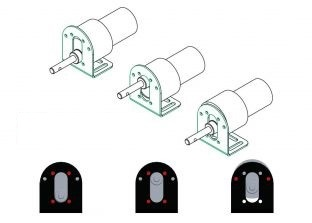
\includegraphics[width=0.8\textwidth]{Sections/LiteratureReview/img/LegAssembly/gearFootMotorMounting.jpg}
    \caption{Multi-height L bracket mounting capability \cite{robu_easymech_nodate}}
    \label{fig:foot_mounting assembly}
\end{figure}


Gear motors operating at 0.6 RPM with 12 Volts DC power,  5.65 Nm torque and 1.2 W are available from McMaster-Carr \cite{mcmaster-carr_gearmotors_nodate}. They have dimensions of L: 3.25 in, W 2.75 in, H: 3 in, and sell for 62.74 USD each.

More heavy duty gear motors are also available from Acklands Grainger \cite{acklands_grainger_dc_nodate}, reaching 80 Nm at 1.3 RPM, 90 Volts DC and 27 Watts. They have dimensions of L: 10 in, W: 2.58 in, H: 4.10 in and weigh 16.0 lbs. They are priced at 821.41 USD each. 
See specifications sheets in Appendices \ref{app:motor_comp_spec}.

\sssubsection{Servo and Stepper Motor} \mbox{}\\
Stepper and Servo motors are heavily used in robotic applications and applications where continuous rotations are not required. Stepper motors have more poles than servo motors, typically 50 to 100 poles, while servo motors only have 4 to 12 poles. Stepper motors are more accurate than servo motors as they can move accurately to their large quantities of poles. Servo motors require encoders to appropriately measure their current location; the servo motor will adjust according to the feedback response of the encoder.  The drawback to having a large quantity of poles, such as for stepper motors, is the reduced torque at high speeds. However, at low speeds the motor will have higher torque capacity compared to a similar size servo motor \cite{amci_stepper_nodate}. Figure \ref{fig:StepperServo} depicts typical shape of a stepper and servo motor.

\begin{figure}[H]
    \centering
    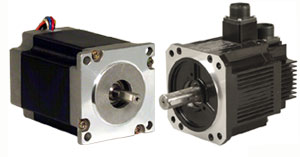
\includegraphics[width=0.9\textwidth]{Sections/LiteratureReview/img/LegAssembly/StepeprServo.jpg}
    \caption{Stepper (Left) vs. Servo (Right) Motor \cite{amci_stepper_nodate}}
    \label{fig:StepperServo}
\end{figure}


The procedure to mount components to the frame can vary based on the component's manufacturer. As shown in Figure \ref{fig:configuration_chassis_mounting}, the servo motor is manufactured with multiple mounting holes, enabling multiple mounting configurations.

\begin{figure}[H]
    \centering
    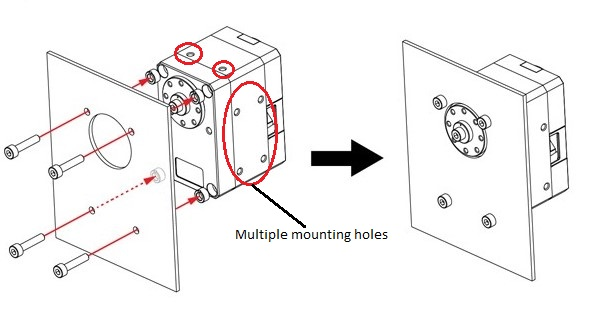
\includegraphics[width=0.9\textwidth]{Sections/LiteratureReview/img/Chasis/Mounting_frame.jpg}
    \caption{Multiple mounting holes \cite{robotis_e-manual_robotis_nodate}}
    \label{fig:configuration_chassis_mounting}
\end{figure}

\sssubsection{Shaft Component Mounting} \mbox{}\\

The mounting or coupling of the motor shaft to the bracket or frame is accomplished through the use of servomotor horns and mounting hubs. Mounting hubs and servo horns have different shapes and forms. However, their mounting mechanism to a shaft is very similar. The horn can be screwed to the spline of the output shaft as shown in Figure \ref{fig:servo-horn}. Mounting hubs can be equipped with set screws to mount to the shaft as shown in Figure \ref{fig:mountinghub_screw}, keyways as shown in Figure \ref{fig:mountinghub_key}, and other shaft coupling mechanisms. The mounting hub can then be linked to other mechanical components such as mechanical linkages, brackets, and more. Commonly, the components are screwed using the screw holes in the servo horn. Figure \ref{fig:servo-horn-linkage} depicts the mounting of a mechanical linkage to the servo horn using a screw, washer, nylon spacer and nut. The nylon spacer functions similarly to a bearing, by enabling the rotation around its axis.

\begin{figure}[H]
    \centering
    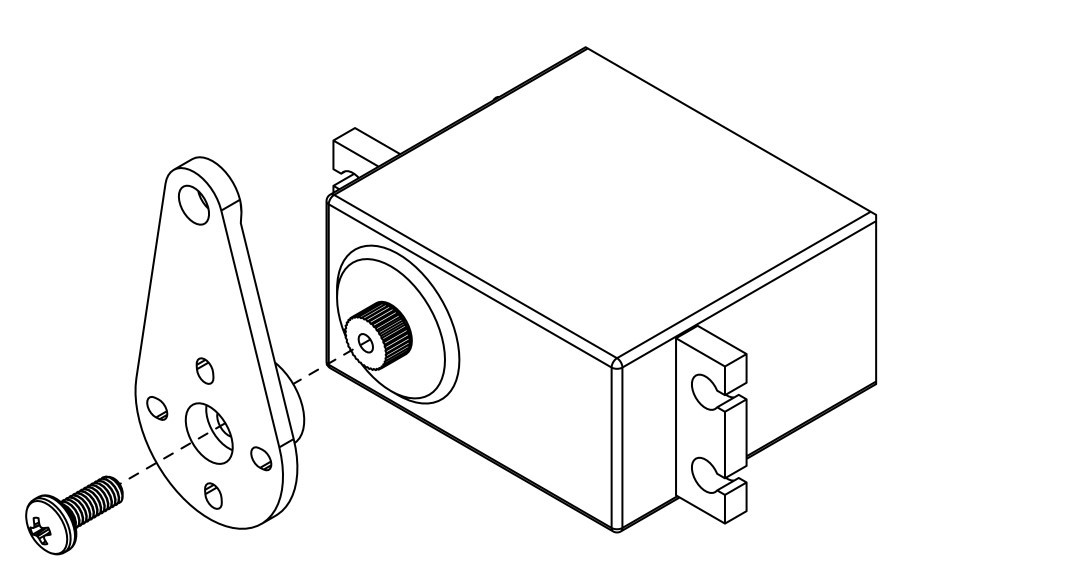
\includegraphics[width=0.5\textwidth]{Sections/LiteratureReview/img/LegAssembly/horn_assembly.jpg}
    \caption{Horn assembly to servo motor \cite{pololu_pololu_nodate}}
    \label{fig:servo-horn}
\end{figure}

\begin{figure}[H]
    \centering
    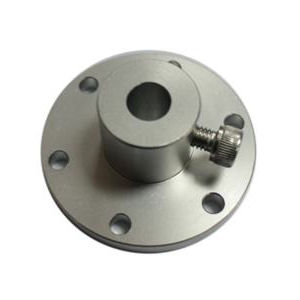
\includegraphics[width=0.4\textwidth]{Sections/LiteratureReview/img/LegAssembly/MountingHub_screw.jpg}
    \caption{Mounting hub with set screw \cite{warbutech_nexus_nodate}}
    \label{fig:mountinghub_screw}
\end{figure}

\begin{figure}[H]
    \centering
    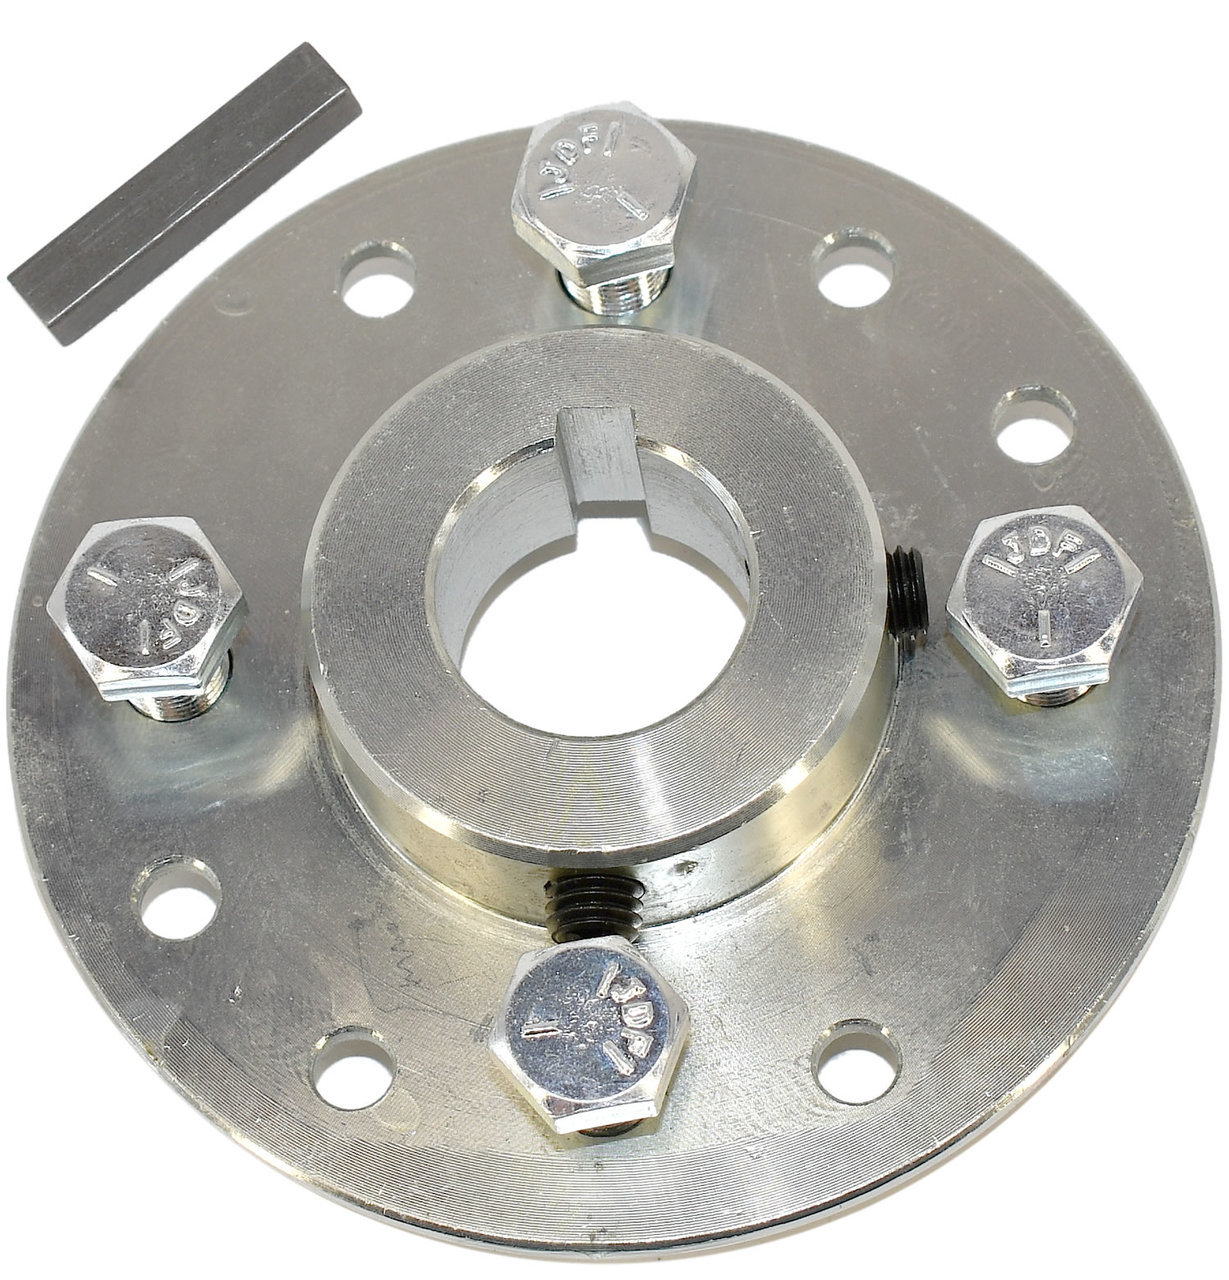
\includegraphics[width=0.4\textwidth]{Sections/LiteratureReview/img/LegAssembly/MountingHub_key.jpg}
    \caption{Mounting hub with key way \cite{gopowersports_sprocket_nodate}}
    \label{fig:mountinghub_key}
\end{figure}

\begin{figure}[H]
    \centering
    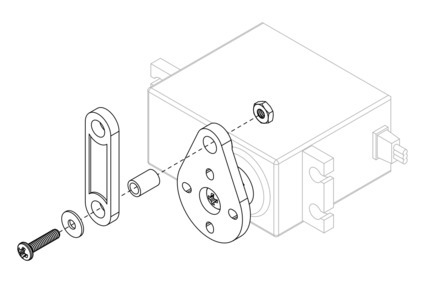
\includegraphics[width=0.7\textwidth]{Sections/LiteratureReview/img/LegAssembly/horn_linkage.jpg}
    \caption{Mounting of mechanical linkage to servo horn \cite{pololu_pololu_nodate}}
    \label{fig:servo-horn-linkage}
\end{figure}

 A two degrees of freedom joint (such as for a hip) can be achieved using two servo motors and a mounting configuration similar to Figure \ref{fig:multi-servo assembly}. The assembly depicted in the Figure \ref{fig:multi-servo assembly} uses a servo mounting bracket and a U shape mounting bracket. The first motor's horn is mounted to a servo motor bracket, the second servo motor is mounted on the bracket, and the second servo's horn is mounted to the U-shape bracket, achieving two degrees of freedom. 

\begin{figure}[H]
    \centering
    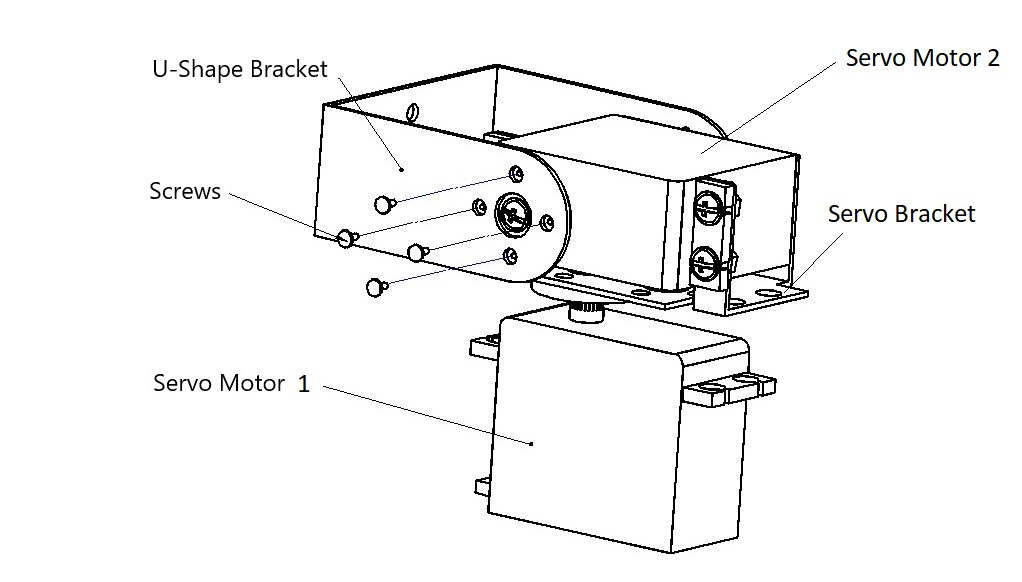
\includegraphics[width=0.9\textwidth]{Sections/LiteratureReview/img/LegAssembly/multi_servo_mounting.jpg}
    \caption{Multi-servo joint typical mounting assembly \cite{pololu_pololu_nodate}}
    \label{fig:multi-servo assembly}
\end{figure}

\subsubsection{Drive System: Other System Types}

Some other drive system options exist which do not fall under the motor and gearbox type. These include belt drive systems and hydraulic systems.

\sssubsection{Belt Drive System}  \mbox{}\\
To transmit power and maximize torque, it is possible to use a belt and pulley system, as seen in the Stanford Doggo design \cite{kau_stanford_2019}. The advantages of this type of system are that it can transmit power between widely spaced shafts, is low cost, is quiet and requires no lubrication \cite{foszcz_basics_2001}. Thus a custom belt drive solution could be useful in transmitting motion to all the legs of the waterfront robot if for example a single central motor was to be chosen. There are various types of belts that can be used, which are separated into two larger categories: friction drive and positive drive. Friction drive belts, such as flat or V-belts, rely on friction. Positive drive belts use teeth which mate with grooves on the pulleys. This allows the belt to keep a more constant speed, as it does not slip \cite{convergence_training_belt_nodate}. This may be required to maintain the full control of the waterfront robot. Figure \ref{fig:drive_belt2} shows the basic components of a belt drive system, and how they are attached to a motor. 

\begin{figure}[H]
    \centering
    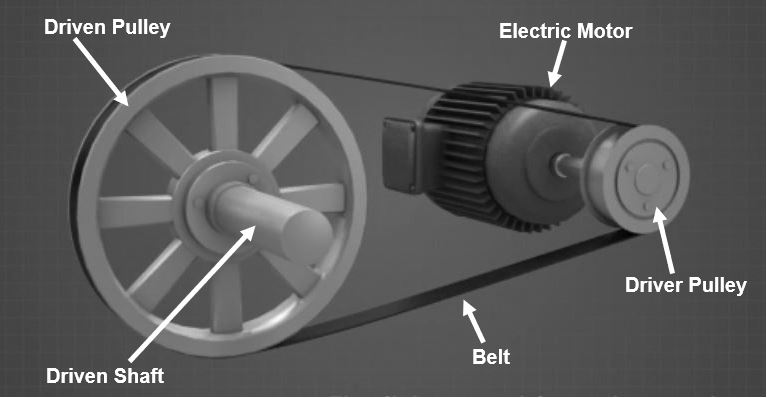
\includegraphics[width=0.9\textwidth]{Sections/LiteratureReview/img/drive/drive_belt2.JPG}
    \caption{Basic components and integration of a belt drive system \cite{convergence_training_belt_nodate}}
    \label{fig:drive_belt2}
\end{figure}

Bushings are used to mount pulleys and sprockets onto shafts. They are available in different formats, including sleeves, quick disconnect and tapper lock formats. Figure \ref{fig:bushing} demonstrates a flange bushing used to mount a pulley to a shaft. The bushing is coupled with the pulley using three screws and mounted on the shaft using a keyway.\cite{machine_design_making_2000}

\begin{figure}[H]
    \centering
    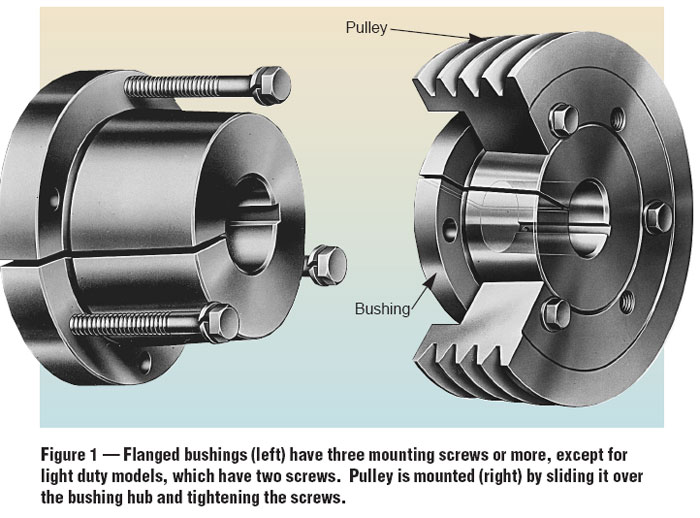
\includegraphics[width=\textwidth]{Sections/LiteratureReview/img/Chasis/Bushing.jpg}
    \caption{Bushing mount for pulley \cite{machine_design_making_2000}}
    \label{fig:bushing}
\end{figure}

\sssubsection{Hydraulic System}  \mbox{}\\

Hamza et al designed a compact hydraulic system capable of fitting on and actuating the MiniHyQ quadruped robot \cite{khan_development_2015-1}.
The system weight is proportional to supply pressure and flow; a reduction in leg velocity also reduces the system weight (a reduction that is amplified by the leg kinematic redundancy found in Figure \ref{fig:minihyq_topology}) \cite{khan_development_2015}.
In the configuration found on MiniHyQ, the power pack occupies 0.59 X 0.2 X 0.19 m of the robots total 0.85 X 0.35 X 0.77 m, weighs 12 kg, has a 13 L/min peak flow rate (10 L/min rated flow rate), 20 MPa operating pressure and 5.5 kW power consumption \cite{khan_development_2015-1}.
The custom design is shown in Figure \ref{fig:minihyq_hydraulic_cad}. It reduces the overall system weight down to 35kg, in contrast to the original HyQ robot's 98kg, for a similar frame size.
Further details on hydraulic power systems can be found in the appendices.

\begin{figure}[H]
    \centering
    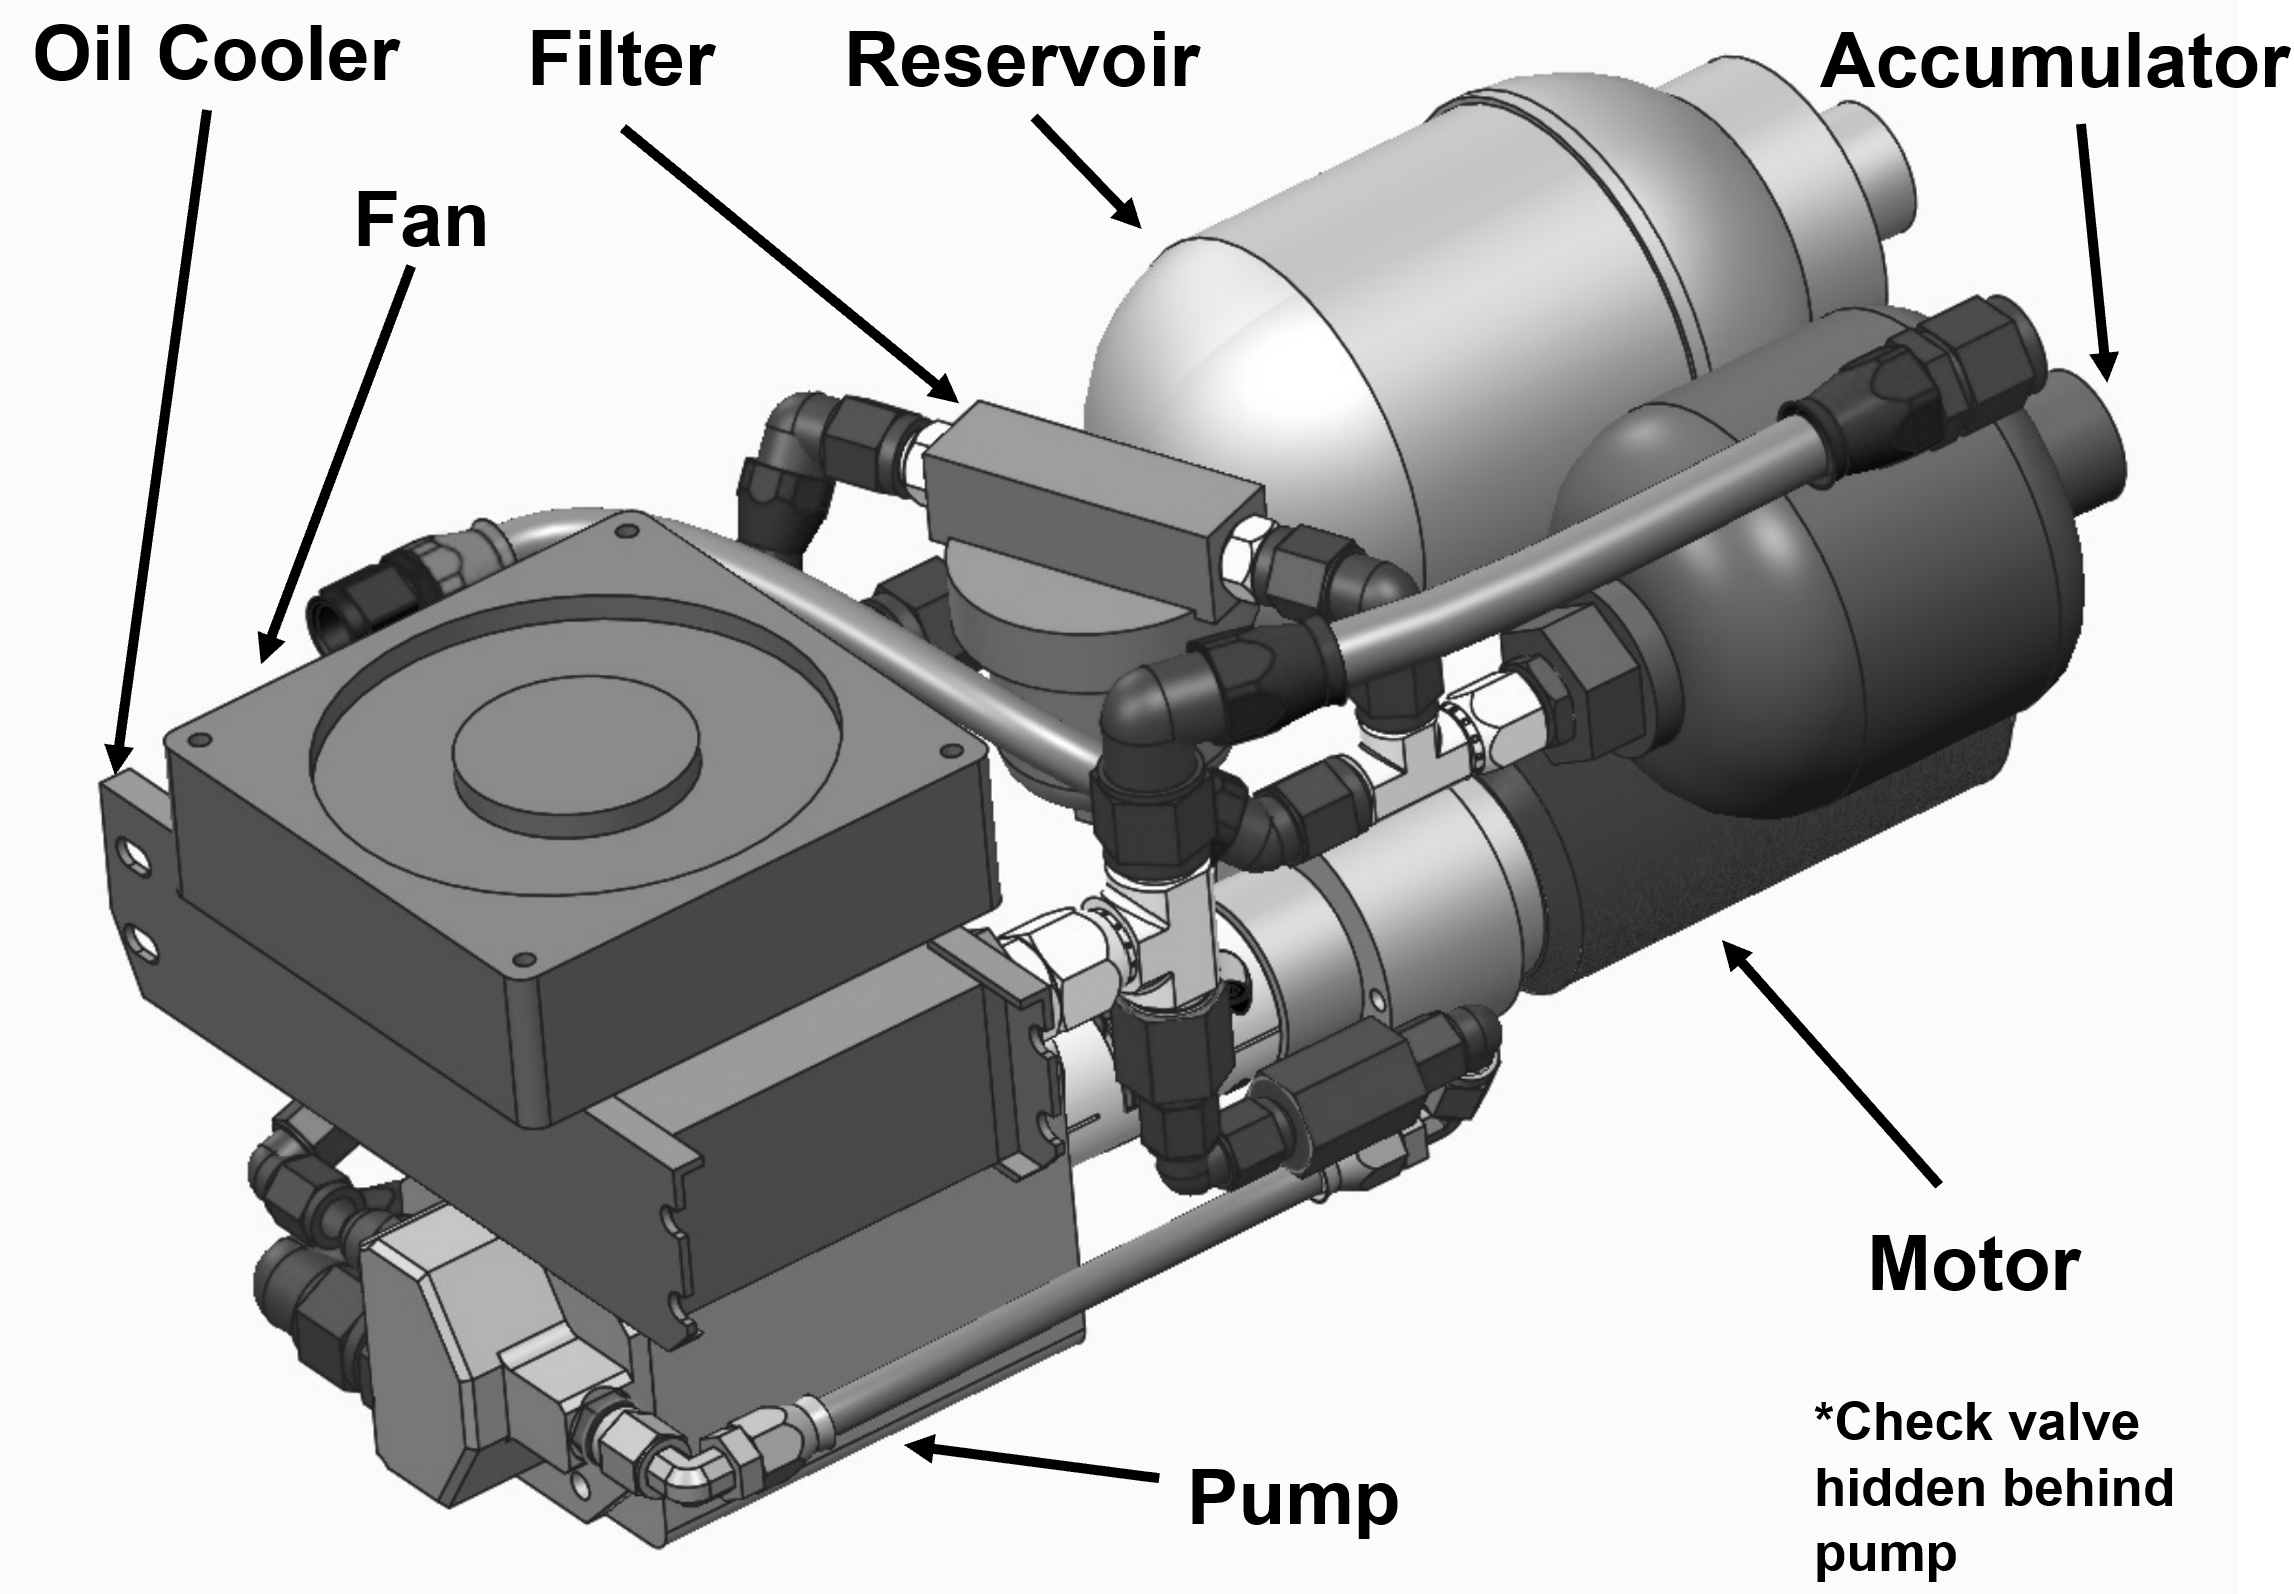
\includegraphics[width=0.8\textwidth]{Sections/LiteratureReview/img/minihyq/subsys_minihqy_hydraulic.png}
    \caption{MiniHyQ on-board hydraulic system \cite{khan_development_2015-1}}
    \label{fig:minihyq_hydraulic_cad}
\end{figure}

%---------------------- COOLING ----------------------%

\subsubsection{Cooling}

Stanford Doggo consumes 840 W at peak; the larger hydraulically actuated MiniHyQ consumes 5.5 kW at peak at 4 times the volume \cite{kau_nate711/stanforddoggoproject_2019} \cite{khan_minihyq_2015}.
Proper cooling for the actuators and electronics is essential for maximizing motor performance \cite{csanyi_optimize_2017}. It is achieved in these robots via passive heating; the robot chassis are open, allowing for airflow to the drivers, computer, and other electronics.
The actuators themselves also have ribbed housings, improving their heat dissipation via natural convection by increasing the surface area exposed to the air.
Both these design decisions are not suitable for a beachfront environment, as all components must be in watertight enclosures.
The simplest solution, passive cooling, is not an option as heat will accumulate in the chassis until components overheat.
Using fans to push heat away from high-power components will not work either, as this simply displaces heat elsewhere in the chassis, with the same result as before.
If moving rapidly, a more well thought-out approach to cooling must be considered.
It was indicated that cooling may not be a necessary design consideration, as the robot will be moving slowly and not output the thousands of watts seen in other dynamic robots.
A detailed look at cooling solutions can be found in the appendices.